\section*{Suggested Reading:}
\begin{itemize}
  \item Principle Component Analysis (PCA): UML 23.1, ESL 14.5
  \item Clustering ESL 14.3
  \item k-means clustering: UML 22.2, ESL 14.3.6
\end{itemize}

\section{Unsupervised learning: Introduction}

So far in his course we worked on {\bf supervised batch learning}, namely the case
where we had a sample space $\X$ and a label / response space $\Y$. We were
interested in {\bf prediction}: how to predict the label $y\in\Y$ corresponding
to a new, unseen
sample $x\in \X$, based on a training set of labeled samples 
$\left\{ (x_i,y_i) \right\}_{i=1}^m$.
\\~\\
However, there are many other kinds of learning problems in the world. Today for
the first time in this course we
will look at problems with a different setup - problems which do not fall into
the framework of supervised batch learning. We'll look at problems where there
is no label $y$ at all! The training data will consist of points
$\left\{ x_i \right\}_{i=1}^m$ with $x_i\in\X$. Learning problems with such data
are called {\bf unsupervised} learning problems.
\\~\\
If you were looking at supervised problems for too long, you may be wondering
what can be done with unlabeled data. Here are three examples:

\begin{enumerate}
  \item {\bf Uncovering low-dimensional structure}

    Sometimes data in $\R^d$ with $d$ large only {\bf appears} to be high-dimensional. Consider a dataset of
    images of the same person looking at different directions. If each image is
    1024-by-1024 pixels (say), then each image lives in $\R^{1024\times 1024}$. (In fact
    even more if the image has color.) 
    But the only degrees of freedom in the dataset is the direction at which t
    person is looking. So we can imagine that this dataset occupies just a 
    very simple subset of $\R^{1024\times 1024}$ - in fact a two-dimensional surface.

    \begin{figure}[H]
      \centering
      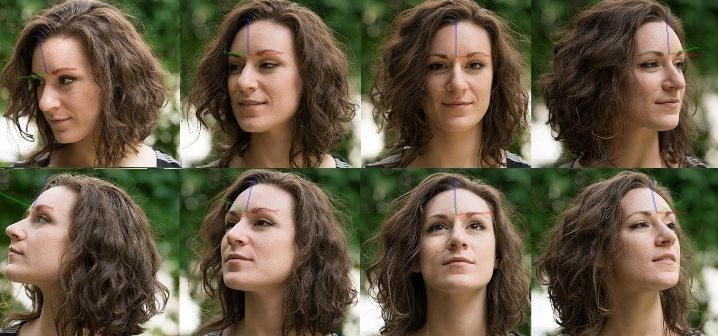
\includegraphics[width=4.5in]{headtrack.jpg}  
          \caption{Head tracking data. (Source: visagetechnologies.com)}
    \end{figure}

    As another example, consider handwritten digits. There are some very famous
    datasets in machine learning of hand-written digits, scanned from 
    zipcodes people wrote on envelopes. Here again each image may be
    28-by-28 pixels, but the data does not occupy the entire space 
    $\R^{28\times 28}$. Instead, there are very few variations on how people write
    digits, and if we allow rotation, translation and dilation of the digit we
    can describe each digit using just a few real numbers. 

\begin{figure}[H]
      \centering
      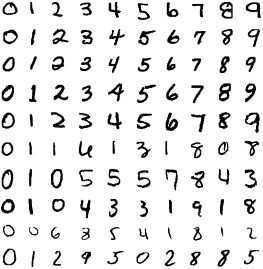
\includegraphics[width=2.5in]{digits.jpg}  
          \caption{Handwritten digits. (Source: Liu et al, Handwritten digit recognition, Pattern
          Recognition 37(2) 2004)}
    \end{figure}
~\\
It would be nice if we could somehow organize the data points in a space that's
smaller and simpler than $\R^{28\times 28}$. For example, it would be nice if we could
have something like this:
%
\begin{figure}[H]
      \centering
      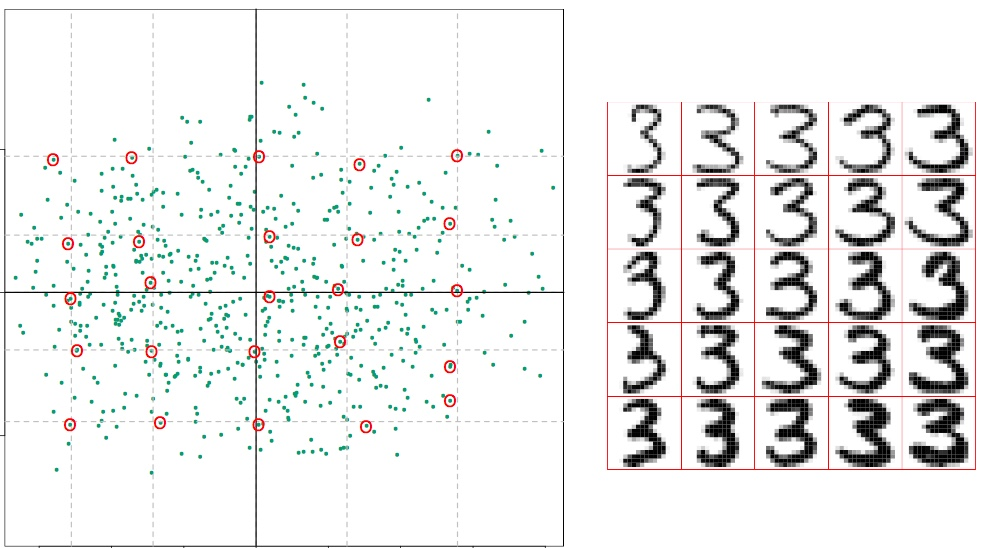
\includegraphics[width=5in]{digit3_pca.jpeg}  
      \caption{Digit 3 in a two-dimensional space. Green dots correspond to
        images of handwritten ``3'' in the dataset. 
        Red circles correspond to
      images shown. (Source: ESL)}
    \end{figure}
~\\
Here,  the handwritten digits ``3'' are all organized on a two-dimensional
    space, meaning that each is determined by just two real parameters, and we
    understand how changing the parameter moves us across the dataset.

    Such a task is called {\bf dimension reduction.} We map each point
    $\V{x}_i$, which lives in a high-dimensional Euclidean space $\R^d$, to a
    point $W(\V{x}_i)$, which lives in a low-dimensional Euclidean space. 
    We use the low-dimensional representation for understanding the structure of
    the dataset; for visualization; for preprocessing; and more.




  \item {\bf Clustering.}

    Suppose now that we obtain a dataset of handwritten digits and want to know
    simply how many different digits are in there, and which images represent
    the same digit. Or suppose we obtain data of a social network and want to
    know how many communities are in there, and the members of each community.
    We don't have labels to help us, and we don't know in advance how many
    digits (or communities) we will find. Such a task is called {\bf
    clustering.} 

    {\bf Another example:} We obtain images of faces, and don't know how many
    different persons there are in the dataset. We would like to know how many
    different persons there are, and group together images that belong to the
    same person. 
    
    \begin{figure}[H]
      \centering
      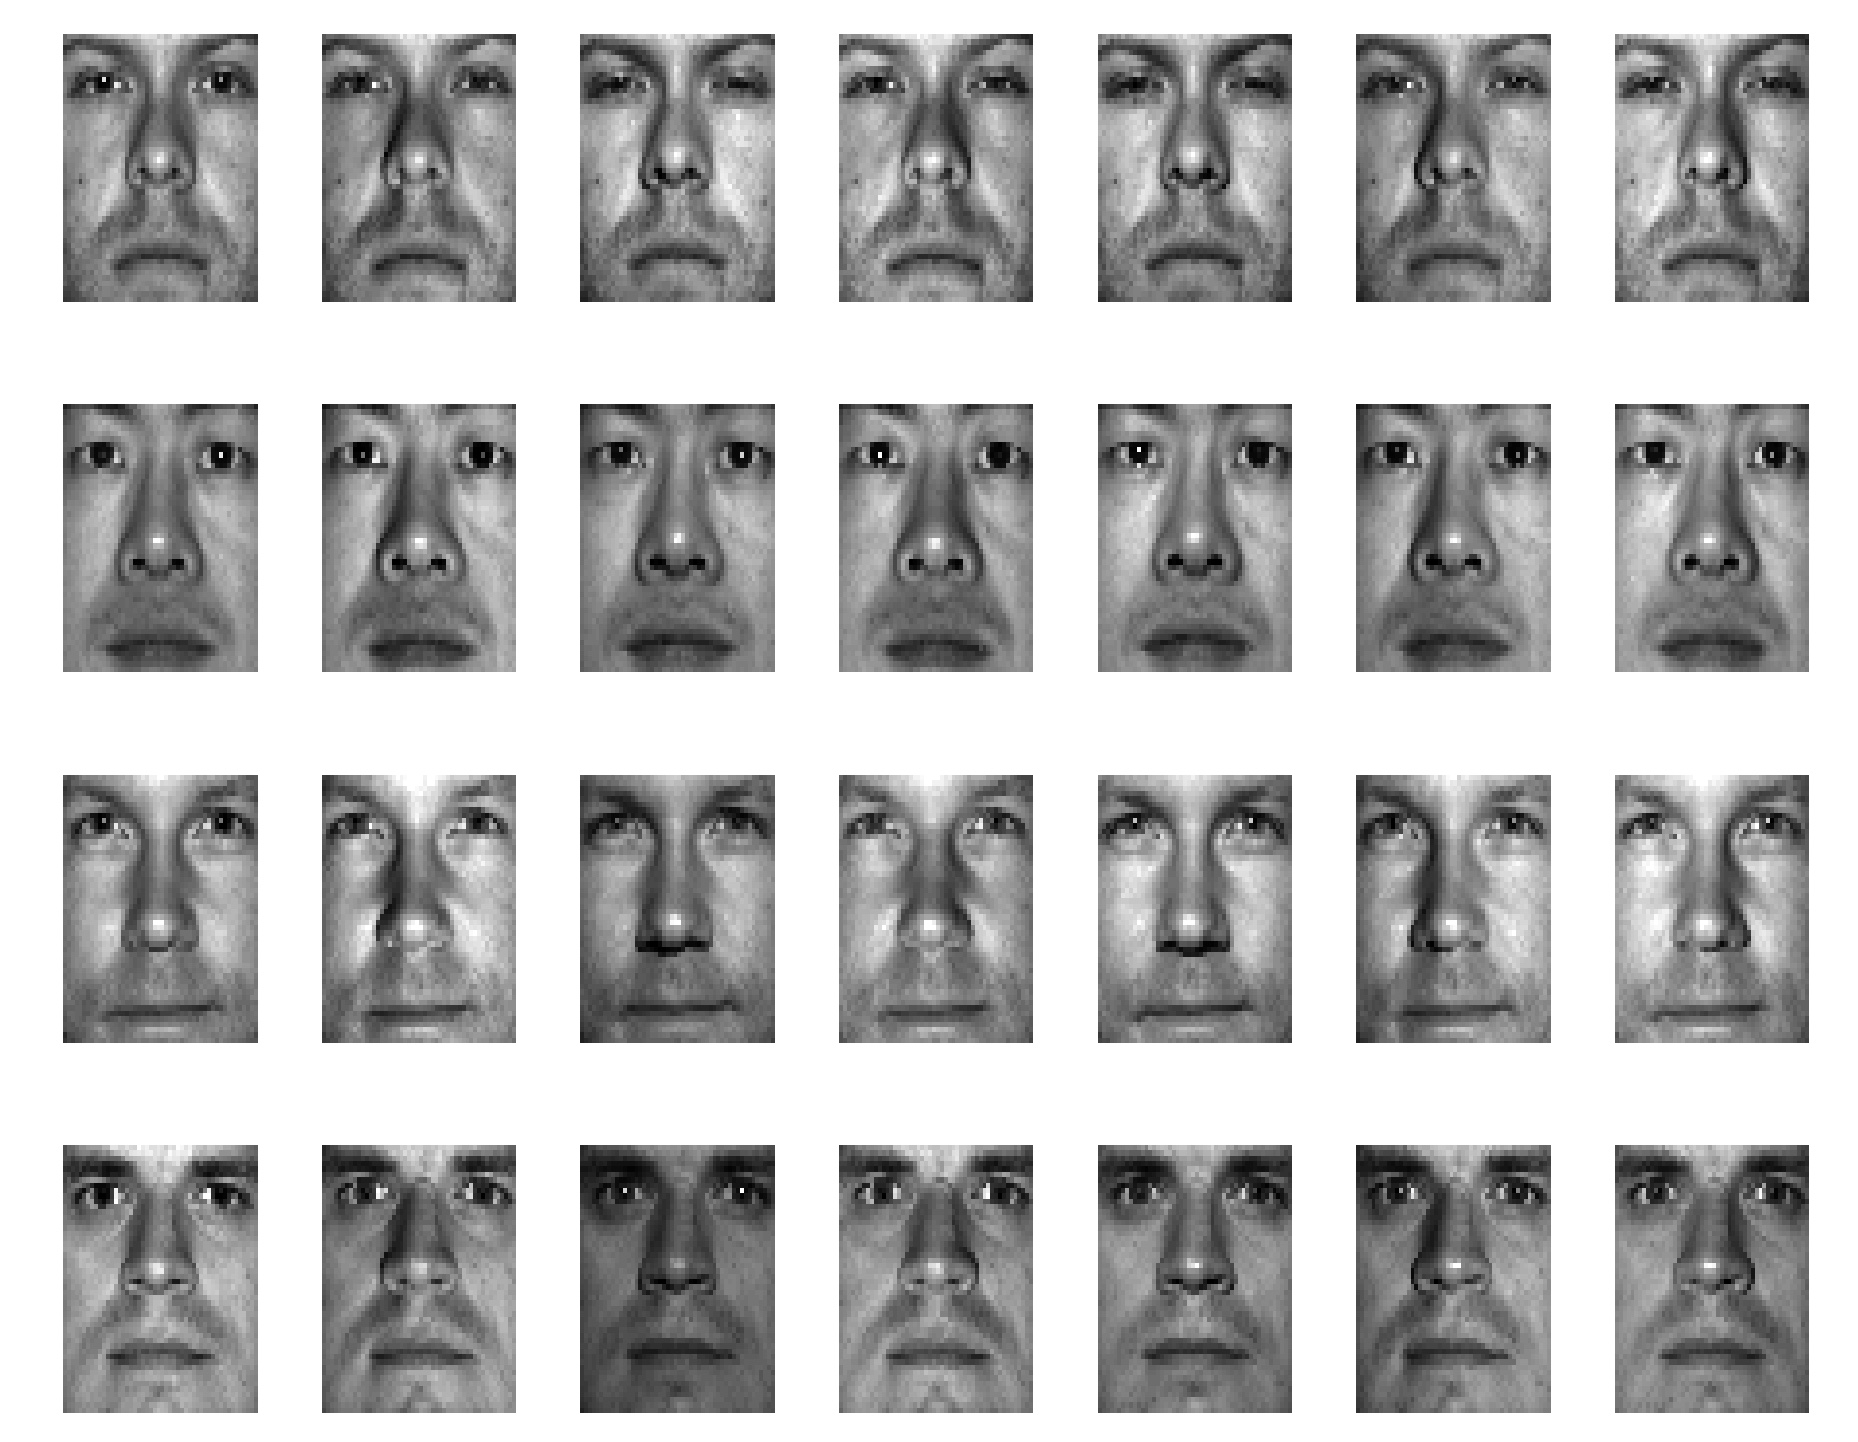
\includegraphics[height=3.5in]{pca_faces_before.jpeg}        
      \caption{Faces of four people from the Yale face dataset}
    \end{figure}

    It would be nice if we could group the images together and count how many
    different people were photographed. 

 \begin{figure}[H]
      \centering
      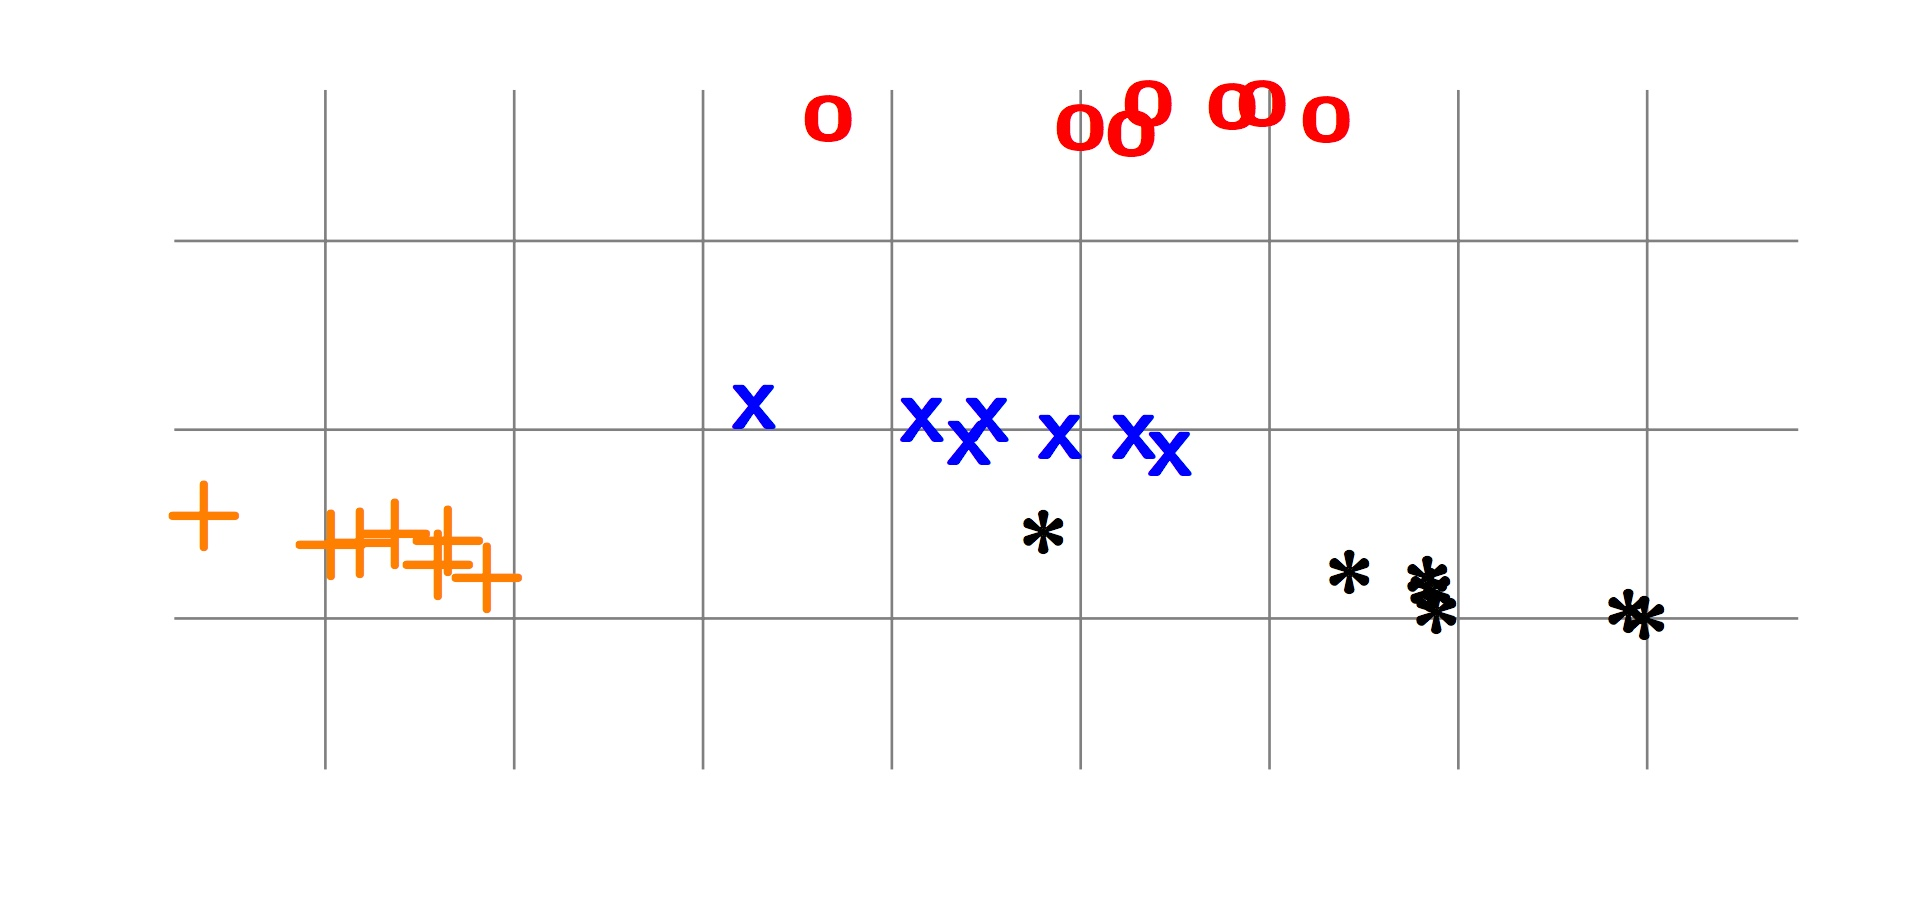
\includegraphics[height=2.7in]{pca_faces_proj.jpeg}        
      \caption{Faces above - dimension reduced to $2$, and clustered. Each of
        the four people is marked with a different marker. (Source:
      UML)} 
    \end{figure}
    ~\\
    So {\bf clustering} means dividing the unlabeled dataset 
    $\{\V{x}_i\}_{i=1}^m$
    into $k$ clusters, where each cluster has something in common (for example,
    each cluster is the same digit, each cluster is the same person, etc) 
    {\bf without using any labels}. 



  \item {\bf Anomaly detection.}

    Another unsupervised learning task has to do with detecting when a system is
    not behaving ``as usual''. Consider an air conditioning system or even a
    power plant. We place sensors in the system and would like to get a warning
    when something is behaving ``strange''. A strange behavior could come from a
    mechanical malfunction, a software problem, or even a cyber-attack - we
    don't know. So we monitor the state of the system all the time. If we have
    $d$ sensors installed, each time we take a reading of the system we get a
    sample $\V{x}_i\in\R^d$. We train our learning systems on readings
    $\V{x}_1,\ldots,\V{x}_m\in\R^d$ where we believe everything was normal. Now
    a new reading comes a long, $\V{x}\in\R^d$. Is it normal? or is there
    something wrong? we are required to make a decision without using any labeled data -
    namely, without having seen the system in a ``wrong'', ``abnormal'' or
    ``strange'' state before.

\end{enumerate}

\subsection{This lecture}

As a brief introduction to unsupervised learning, we will see 
\begin{itemize}
  \item The simplest, most
popular method for dimension reduction: {\bf Principal Component Analysis} 
(PCA)
\item The simplest, most popular method for clustering: {\bf $k$-means
  clustering.}
\end{itemize}


\section{Dimension reduction}

Let $\V{x}_1,\ldots,\V{x}_m\in\R^d$ be our dataset. 
In dimension reduction we are looking for a map $W:\R^d\to\R^k$ (with $k<d$)
such that anything we would like to do with $\V{x}_1,\ldots,\V{x}_m$
we can do, in some sense, with 
$W(\V{x}_1),\ldots,W(\V{x}_m)$. When the map $W$ is a linear map, this is
called {\bf linear dimension reduction.}
When $W$ is non-linear, this is called {\bf nonlinear dimension reduction.}
In this lecture we'll only think about linear dimension reduction.
\\~\\
There are many reasons to study dimension reduction:
\begin{itemize}
  \item {\bf Learning:} As we have seen, some learning algorithms on $\R^d$ 
    work better
    when the dimension $d$ is small compared with the training sample size $m$,
    and some fail if $d$ is too large.

  \item {\bf Visualization:} If we can reduce dimension to $k\leq 4$ then we can
    plot the data on a page (possibly on a 3-dimensional axis. The forth
    dimension can be represented by color).
  \item {\bf Computation:}
    As we have seen, the time and space complexity of many learning algorithms
    grows with the dimension $d$. By reducing dimension as part of our
    preprocessing, we can use fewer computational resources for the same task.
\end{itemize}

\subsection{Linear dimension reduction}

Suppose that our dataset is 
$\V{x}_1,\ldots,\V{x}_m\in\R^d$ where $d$ is large. But suppose that our
data do not actually occupy the entire
space $\R^d$. Suppose instead that they live on a $k$-dimensional linear 
subspace of $\R^d$, or very close to a  $k$-dimensional linear 
subspace:

\begin{figure}[H]
  \centering
  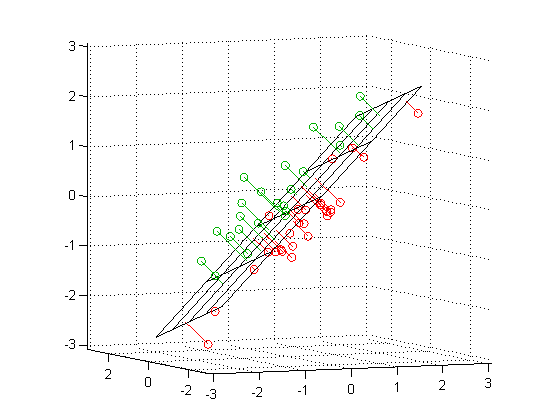
\includegraphics[height=2.5in]{subspace.png}    
  \caption{Data close to a linear subspace of $R^d$}
\end{figure}

It would make sense to somehow project the data to this subspace and choose the
map $W:\R^d\to\R^k$ accordingly. 
But there are two
problems: 
\begin{enumerate}
  \item We don't know this subspace. We just have the data. We need to find a
    basis for this subspace.
  \item Even if we knew the subspace, 
    simply projecting a point $\V{x}\in\R^d$ onto this subspace does not 
    reduce dimension: the projected point is still in $\R^d$. What we actually
    want is to find an orthonormal basis for this subspace, and then find
    the $k$ coordinates of 
    projected point according to the subspace. This would result in $k$ 
    real numbers, so would mean we indeed reduced dimension to $k$. 
 
\end{enumerate}
~\\
So we see that the problem of linear dimension reduction means finding an
orthonormal basis for the subspace that best approximates the training data. Can
this be done?

\subsection{Principal Components Analysis (PCA)}

PCA is the most well-known {\bf linear} dimension reduction method. 
We choose $k$ (the reduced dimension) and  look
for a linear map $W:\R^d\to\R^k$. How shall we choose $W$? With $W$ we will also
look for an ``inverse'' map $U:\R^k\to\R^d$, mapping the reduced points back to
the original space $\R^d$. Let's measure the error incurred by the whole process
using sum of squares
\[
           \sum_{i=1}^m\norm{\V{x}_i - UW\V{x}_i}^2
         \]
which we seek to minimize.
\\~\\
{\bf The PCA problem} is therefore:
Given points $\x_1,\ldots,\x_m\in\R^d$, find
\[
  \argmin_{W \in \reals^{k,d}, U \in \reals^{d,k}} \,\,\sum_{i=1}^m \|\x_i - U W
\x_i\|^2\,.
\]
~\\
{\bf Theorem. (The solution to the PCA problem.)}
Let $A = \sum_{i=1}^m \x_i \x_i^\top$ and let $\u_1,\ldots,\u_n$ be the $n$
leading eigenvectors of $A$. Then, the solution to the PCA problem is as
follows.  
Let $U$ be the $m$-by-$k$ matrix whose columns are 
$\u_1,\ldots,\u_k$ and let $W = U^\top$. Then $U$ and $W$ solve the PCA
problem for $\x_1,\ldots,\x_m$.
~\\
{\bf Proof.}
\begin{itemize}
  \item $UW$ is a $d$-by-$d$ matrix of rank $k$, therefore its image space 
    is subspace of $\R^d$ whose dimension is at most $k$.
    Let us denote this subspace by $S=Im(UW)$.
  \item The transformation $\x \mapsto UW\x$ moves $\x$ to the subspace $S$.
  \item Thefore the quantity 
    $\norm{\V{x}_i - UW\V{x}_i}^2$ is minimized if and only if we choose $U$ and
    $W$ such that $UW$ is an orthogonal projection on $S=Im(UW)$.
  \item The point in $S$ which is closest to $\x$, namely the orthogonal
    projection of $x$ on $S$, is given by $V V^\top \x$, 
    where the columns of $V$ span an orthonormal basis of $S$.
\item Therefore, we can assume w.l.o.g. that $W = U^\top$ and that 
  the columns of
  $U$ are orthonormal.
\item Now observe that 
\[
\begin{split}
\|\x - U U^\top \x\|^2 &= \|\x\|^2 - 2 \x^\top U U^\top \x + \x^\top U
U^\top U U^\top \x \\
&= \|\x\|^2 - \x^\top U U^\top \x \\
&= \|\x\|^2 - \mathrm{trace}(U^\top \x \x^\top U) ~,
\end{split}
\]
\item Therefore, an equivalent problem to the PCA problem is
\[
\argmax_{U \in \reals^{d,k} : U^\top U = I} \mathrm{trace}\left(U^\top
\left(\sum_{i=1}^m \x_i \x_i^\top \right) U\right) ~.
\]
\item Denote $A = \sum_{i=1}^m \x_i \x_i^\top$. Then we need to solve
\[
\argmax_{U \in \reals^{d,k} : U^\top U = I} \mathrm{trace}\left(U^\top
\cdot A \cdot U\right) ~.
\]
\item A is symmetric and in fact positive semidefinite. 
  Now let $A=VDV^\top$ be the spectral decomposition of $A$, where the diagonal
  of $D$ are the eigenvalues of $A$ in decreasing order and the columns of $V$
  are the corresponding eigenvectors. 
\item Now comes the following claim: 
  for any $d$-by-$k$ orthonormal matrix $U$, we have
  \[
 \mathrm{trace}\left(U^\top
 \cdot A \cdot U\right) \leq \sum_{i=1}^k D_{i,i}\,.
  \]
 % let $B=V^\top U$ and observe
 % that
 % \[
 %   U^\top A U = B^\top D B\,.
 % \]
  (See proof in UML page 325). Observe that the bound on the right hand side 
  is just the sum of the $k$ leading eigenvalues of $A$.
\item But if we take $U$ to be $\tilde{U}$, the $m$-by-$d$ matrix whose columns are the $k$
  leading eigenvectors of $A$, then $U$ is orthonormal and 
 \[
   \mathrm{trace}\left(\tilde{U}^\top
   \cdot A \cdot \tilde{U}\right) = \sum_{i=1}^k D_{i,i}\,.
 \]
  $\blacksquare$
\end{itemize}


\subsection{PCA as Variance Maximization}

Actually, there is no reason why the linear subspace, on which (or close to
which) the data points are located in $\R^d$, should go through the origin. In
other words, we would like to allow the map $W$ to be {\bf affine} (meaning a
linear transformation plus a constant, an intercept) - not just linear.
So let's generalize the above and consider $W:\R^d\to\R^k$ to be of the
form $W(\V{x}) = \tilde{W}(\V{x}-\mu)$ where $\mu\in\R^d$ and
$\tilde{W}:\R^d\to\R^k$ a linear map.  This allows us to
``shift'' the data before applying the linear map $\tilde{W}$. 
It turns out that if we add an optimization also over $\mu$ to the PCA problem,
then the best $\mu$ is given by 
\[
  \overline{\V{x}} = \frac{1}{m}\sum_{i=1}^d \V{x}_i
\]
(see ESL 14.5.1). Note that this is just the empirical mean of the data. 
\\~\\
Making this change, we see that the matrix $A$ above is now defined as

\[
  A = \sum_{i=1}^m (\x_i-\overline{\V{x}}) (\x_i-\overline{\V{x}})^\top
\]
instead of
$A = \sum_{i=1}^m \x_i \x_i^\top$.
We recognize this matrix as the {\bf sample covariance}! We thus become curious
if there is some connection between PCA and variance / covariance of the data.
\\~\\
Not  surprisingly, there is. In the recitation you'll see how PCA can also be
derived by looking for a set of orthogonal 
directions along which the variance of the data is maximized. This is a
different derivation leading to the same algorithm we have found 
(namely, diagonalizing the
empirical covariance matrix and projecting the data on its $k$ 
leading eigenvectors). In that derivation we effectively decompose the empirical
covariance matrix $A$ to its eigenvector, where each eigenvector represents a
different component of the covariance.

\subsection{PCA - formal definition.}

So let's write a formal definition of the Principal Components Analysis.
With some minor missing steps, we have proved:
\\~\\
 {\bf Theorem:} Suppose we decide to reduce from dimension $d$ to
 dimension $k$ using a linear dimension reduction, and measure the quality of
 dimension reduction with sum of squares. Then
            \[
              \text{argmin}_{U,W} \sum_{i=1}^m\norm{\V{x}_i - UW\V{x}_i}^2
         \]
         over matrices $U\in\R^{d\times k}$ and $W\in\R^{k\times d}$
         is achieved when the columns of $U$ are the first $k$ eigenvectors of
         the sample covariance matrix 
         \[
           S = \frac{1}{m}\sum_{i=1}^m (\V{x}_i-\overline{\V{x}}) 
           (\V{x}_i -\overline{\V{x}})^\Tr
         \]
         and $W=U^\Tr$.
\\~\\
 {\bf Definition:} Let
         be the sample covariance matrix of the training data
         $\V{x}_1,\ldots,\V{x}_m$ as above.
         Let $\V{u}_1,\ldots,\V{u}_d$ be the eigenvectors of $S$ corresponding
         to eigenvalues $\lambda_1,\ldots,\lambda_d$, ordered such that
         $\lambda_1\geq \lambda_2\geq \ldots \geq \lambda_d\geq 0$.


        \begin{itemize}
          \item The number $\lambda_i$ is called the {\bf $i$-th Principal
            Value} of  $\V{x}_1,\ldots,\V{x}_m$.
          \item The vector $\V{u}_i$ is called the {\bf $i$-th Principal
            Vector} of  $\V{x}_1,\ldots,\V{x}_m$.
        \end{itemize}
~\\
Since the empirical covariance $S$ is  a $d$-by-$d$ positive semidefinite
matrix, its eigenvectors $\V{v}_1,\ldots, \V{v}_d$ (which we called the Principal Components) form an
orthonormal basis for $\R^d$. 
\\~\\
{\bf Definition:} Fix $k$. 
The PCA dimension reduction to $k$ dimensions maps each point
$\V{x}_i$ to
$U^\top \V{x}_i$, where the columns of $U$ are the $k$ leading principal
vectors $\V{v}_1,\ldots,\V{v}_k$.
{\bf Note that $U^\top \V{x}_i$ is just the vector of $k$ coordinates of
$\V{x}_i$ according to $\V{v}_1,\ldots,\V{v}_k$,} namely, the
  coordinates of the projection of $\V{x}_i$ onto the optimal subspace, 
  which is given by $Span\left\{ \V{v}_1,\ldots,\V{v}_k \right\}$.

\subsection{Applying PCA dimension reduction to an arbitrary vector in $\R^d$}
As $\V{v}_1,\ldots, \V{v}_d$  (the principal vectors) are an orthonormal basis
for $\R^d$, we have the following:
\begin{enumerate}
  \item Any data point $\V{x}\in\R^d$ can be written as a linear 
    combination of  $\V{v}_1,\ldots, \V{v}_d$. 
  \item Let $\V{x}=\sum_{i=1}^d \inner{\V{x},\V{v}_i}\, \V{v}_i$ be the unique decomposition
    of some point
    $\V{x}\in\R^d$ - not necessarily in our training 
    dataset -  on the principal components. 
    We've seen that for each $k<d$, the best linear dimension reduction of
    $\V{x}_i$ ($i=1,\ldots, m$) in the least squares sense above, is 
    given by the column vector $(\inner{\V{x},\V{v}_1},
    \ldots,
  \inner{\V{x},\V{v}_k})^\top$. 
    We can use this map on any other vector $\V{x}$ and reduce its dimension
    with the same linear map, mapping it to 
    the column vector $(\inner{\V{x},\V{v}_1},\ldots,
      \inner{\V{x},\V{v}_k})^\top\in\R^k$.
    So while the subspace we project on corresponds to the training sample 
    $\V{x}_1,\ldots,\V{x}_m$, and the linear dimension reduction is optimal for
    these points, we can use it for any point in $\R^d$. 

\end{enumerate}


\subsection{The subtle difference between the projected points and their
coordinates.}

It is very important to understand the difference between 
the projection on the span of the first $k$ principal vectors (projection on the
optimal subspace) and the coordinates of that projection according to the
principal vectors.
\\~\\
Suppose for a moment that $d=3$ and $k=2$. When we run PCA on
$\V{x}_1,\ldots,\V{x}_m\in\R^3$, we find a two-dimensional subspace and project
each $\V{x}_i$ on that subspace. The best subspace is the one that minimizes the
sum of squared distances between each $\V{x}_i$ and its projection. As we just
proved, it is spanned by the two leading eigenvectors of the $3$-by-$3$ matrix
$
           S = \frac{1}{m}\sum_{i=1}^m (\V{x}_i-\overline{\V{x}}) 
           (\V{x}_i -\overline{\V{x}})^\Tr\,.
         $
\\~\\
Now, we are not just interested in projecting the points in $\R^3$ 
on the 2-dimensional subspace  spanned by these two leading eigenvectors.
We would like to actually reduce dimension, namely, find the map 
$W:\R^3\to \R^2$ and work with the dimension-reduced dataset  
$W(\V{x}_1),\ldots,W(\V{x}_m)$. As we proved above, 
in fact $W=U^\top$ where the columns of
$U$ are the two leading eigenvectors of $A$ (taken to be orthonormal, since $A$
is positive semidefinite). So the dimension-reduced version of the point
$\V{x}_i\in\R^d$ is just
$U^\top \V{x}_i$ - the {\bf coordinates} of the vector $\V{x}_i$ according to the
orthonormal set of $k$ leading eignevectors of $A$. 
\\~\\
If $\V{v}_1,\V{v}_2,\V{v}_3$  are all three principal components (so that the
two leading ones are $\V{v}_1$ and $\V{v}_2$) then 
a vector $\V{x}_i$ in our data decomposes as
$\V{x}=\sum_{i=1}^3 \inner{\V{x},\V{v}_i}\, \V{v}_i$. 
The {\bf projection}
of $\V{x}_i$ on the optimal two-dimensional subspace 
is given by 
$\V{x}=\sum_{i=1}^2 \inner{\V{x},\V{v}_i}\, \V{v}_i$, while the 
{\bf coordinates}
of $\V{x}_i$ according to the two leading principal vectors are
given by $(\inner{\V{x},\V{v}_1},\inner{\V{x},\V{v}_2})$. In matrix form, these
coordinates are given by $U^\top \V{x}_i$ where the first column of $U$ is
$\V{v}_1$ and the second column of $U$ is $\V{v}_2$.
\\~\\
The difference between the projected point (which is still a point in $R^3$) and
the two coordinates according to the orthonormal basis spanning the subspace is
made clear in the following image:
\begin{figure}[H]
  \centering
  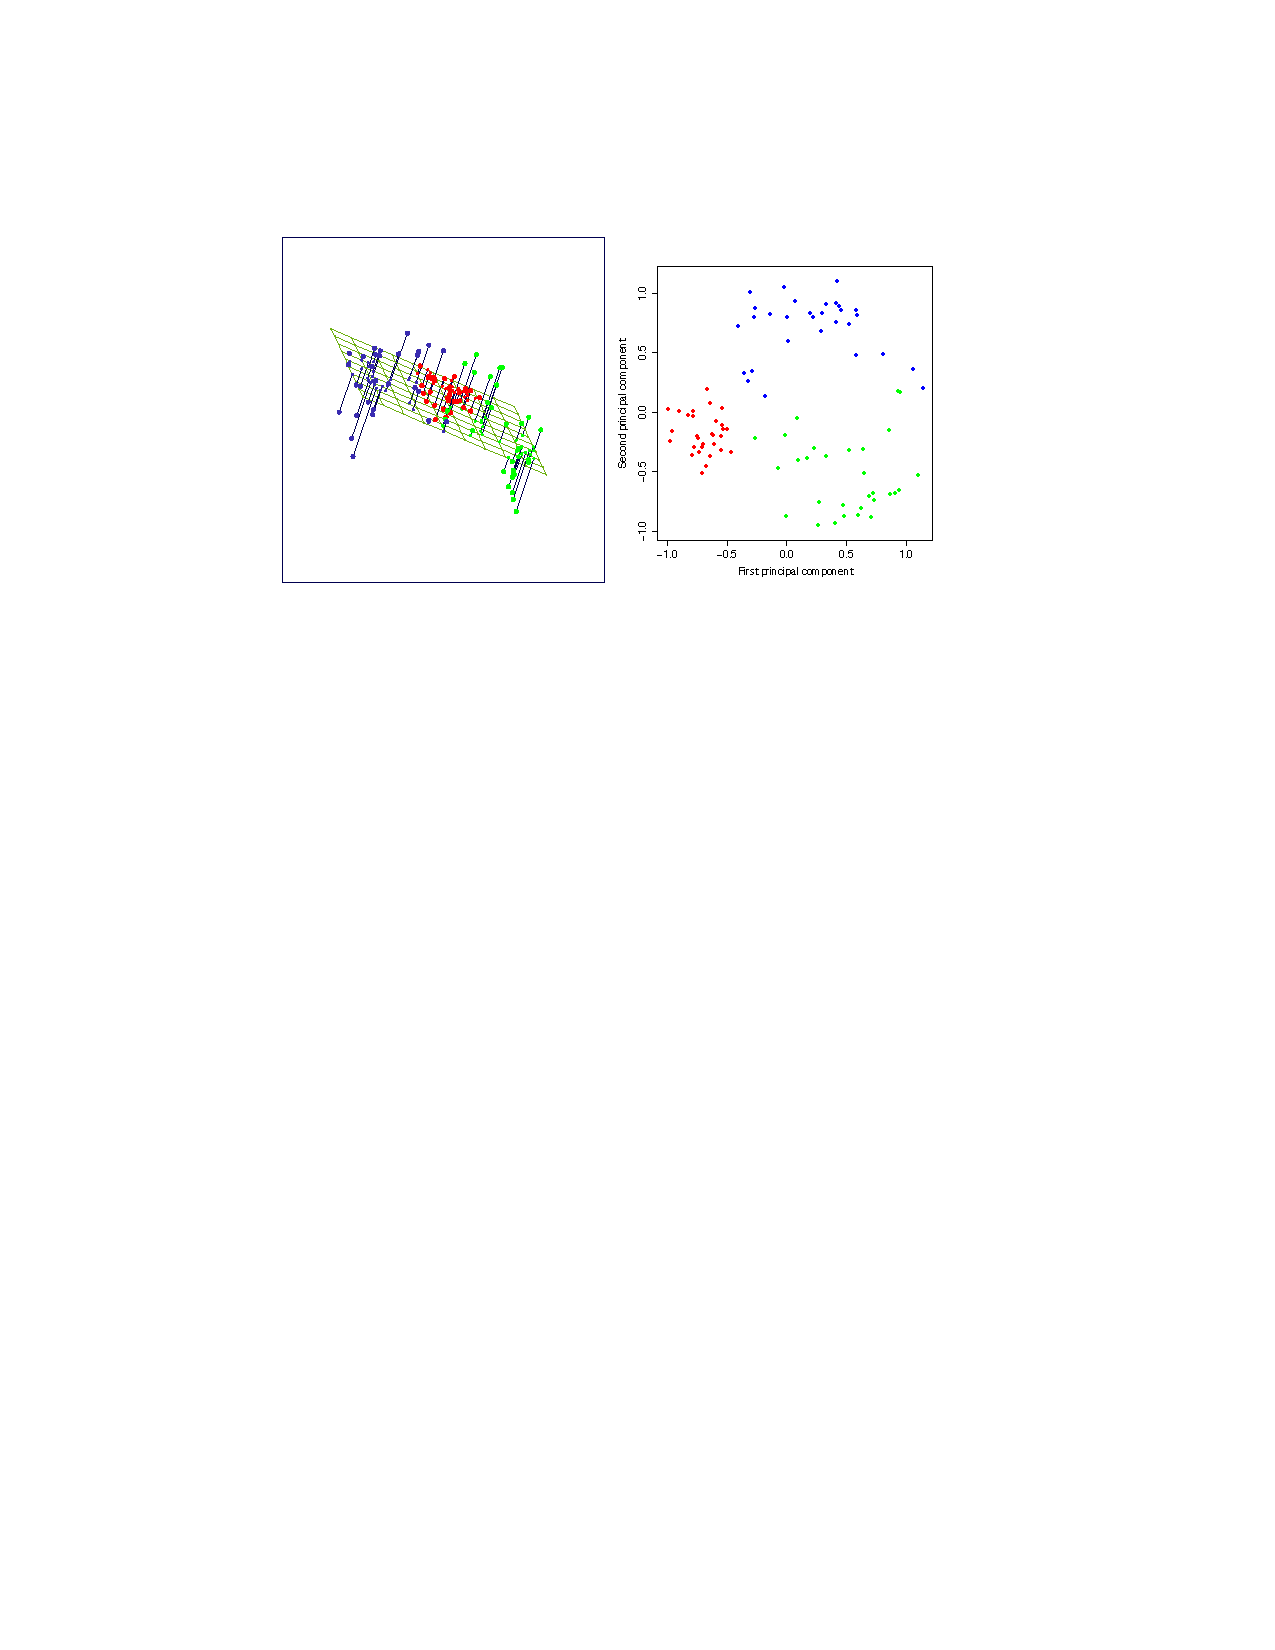
\includegraphics[height=2.5in]{pca_proj_colors.pdf}    
  \caption{Left: points $\V{x}_1,\ldots,\V{x}_m$ are projected on the 
  subspace spanned by the two leading eigenvectors of $A$. Right: coordinates of
the projected points according to these two orthonormal vectors. (Source: ESL)}
\end{figure}
~\\
If you don't fully grasp the difference between the left panel and the right panel,
PCA may remain a mystery to you. Spend time making sure you understand the
difference.
\\~\\
(Recall our lecture on linear regression, where we first projected a vector on a
subspace, and then looked for the coordinates of the projected point according
to a set of vectors spanning the subspace. There, the spanning set was usually
not orthonormal. Here, it is always orthonormal.)

Here is another example for $d=3$ and $k=2$. The dataset (left panel) 
is a point cloud in
$\R^3$ shaped like a bagel. In the dimension-reduced dataset in $\R^2$ we
replace each point with the {\bf coordinates} of its projection on the
two-dimensional ``principal subspace'' $Span\left\{ \V{v}_1,\V{v}_2 \right\}$.
\begin{figure}[H]
  \centering
  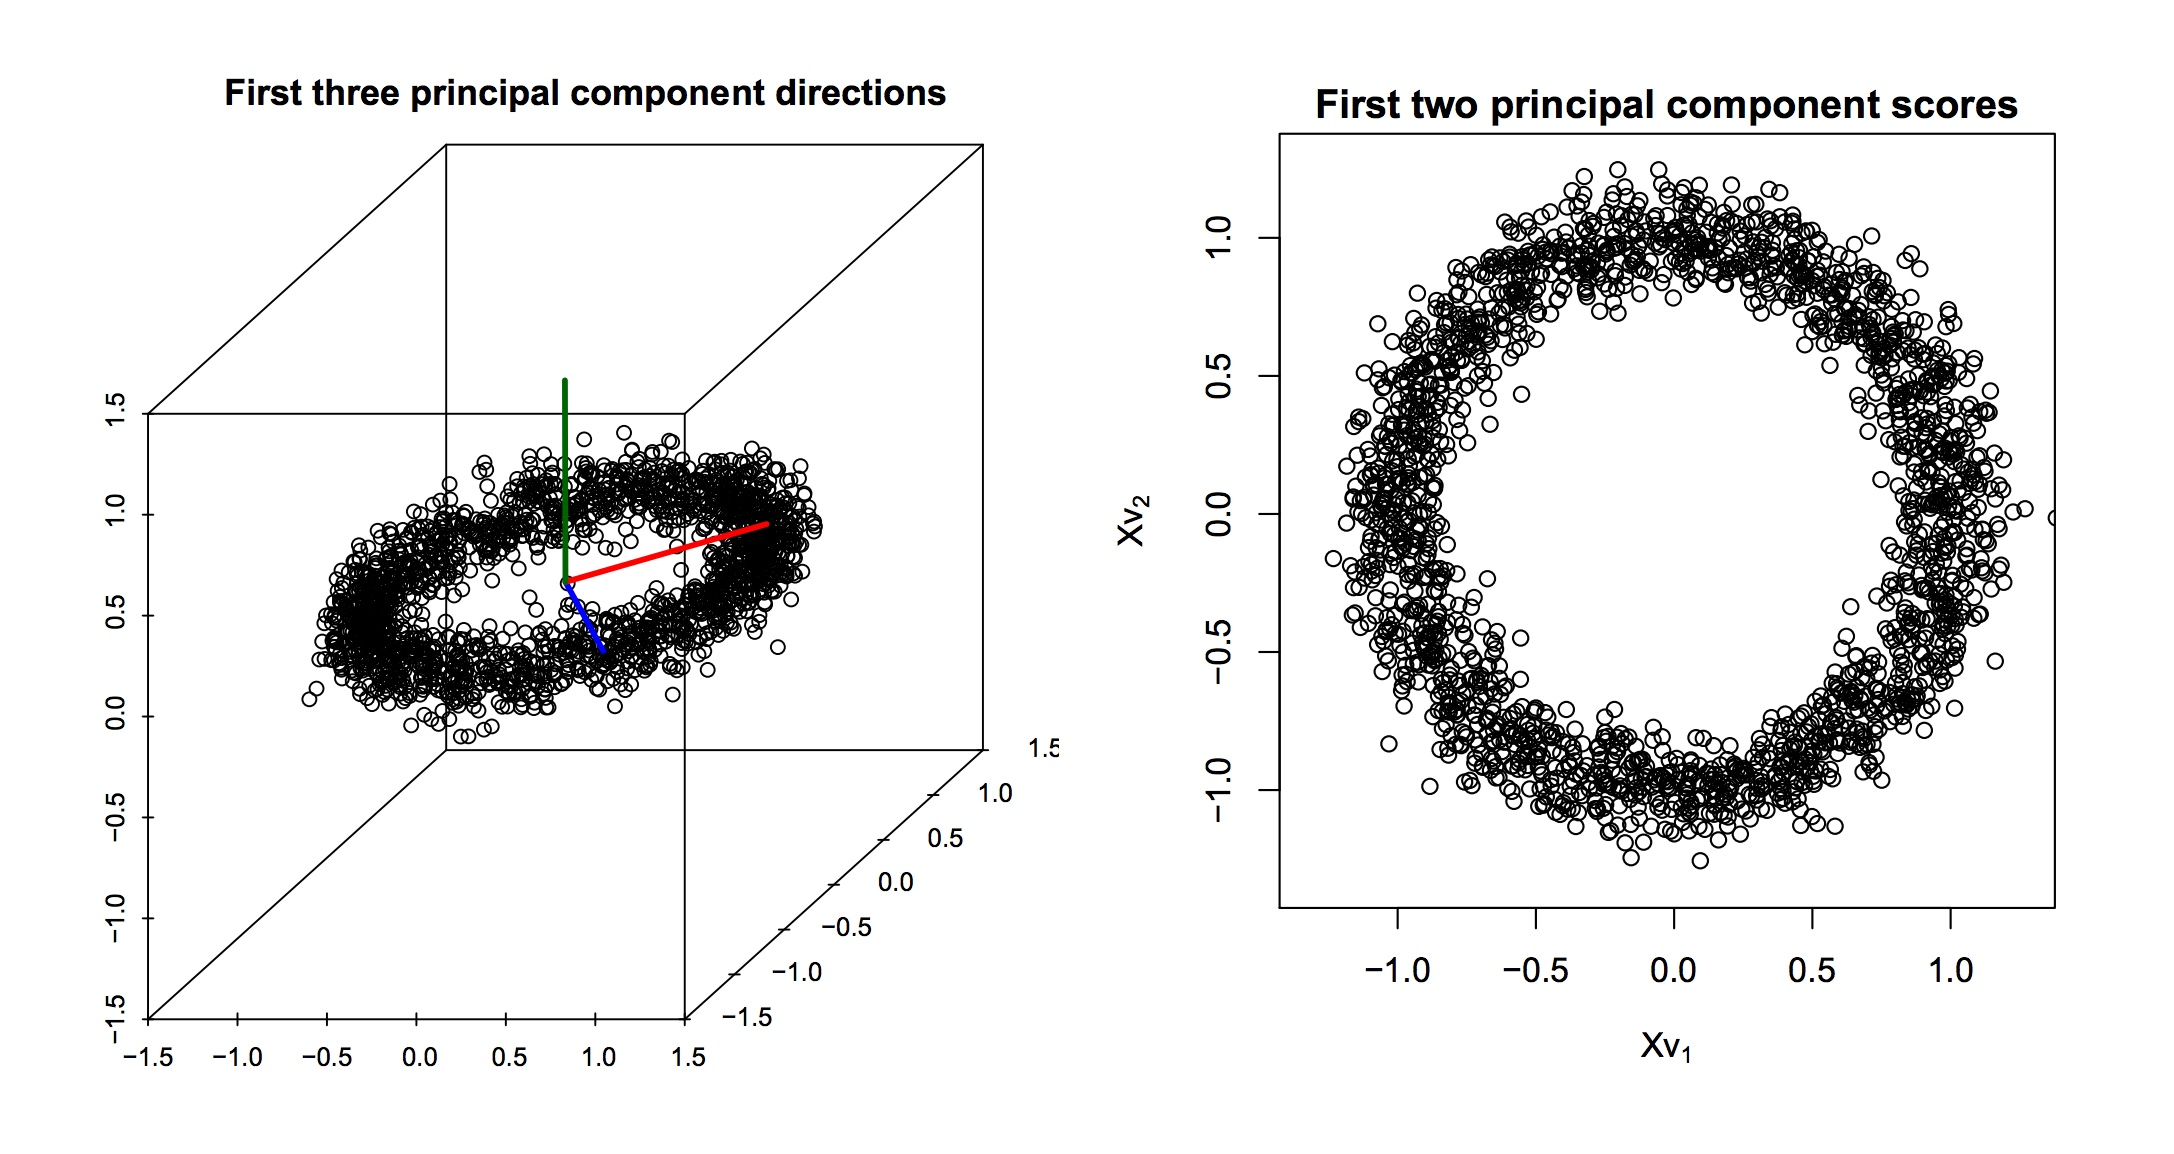
\includegraphics[height=2.5in]{pca_tib_1.jpeg}    
  \caption{(Source: CMU 36-462/36-662)}
\end{figure}
~\\
In contrast, look at the figure below. We can look at the {\bf projection} of the bagel dataset on the
principal subspace for $k=1$ (left panel), $k=2$ (middle panel) 
and $k=3$ (right panel). All these sets are point clouds in $\R^3$. There is not
dimension reduction here. Of course,
for $k=3$ we project on the whole space, so we get the original dataset.
\begin{figure}[H]
  \centering
  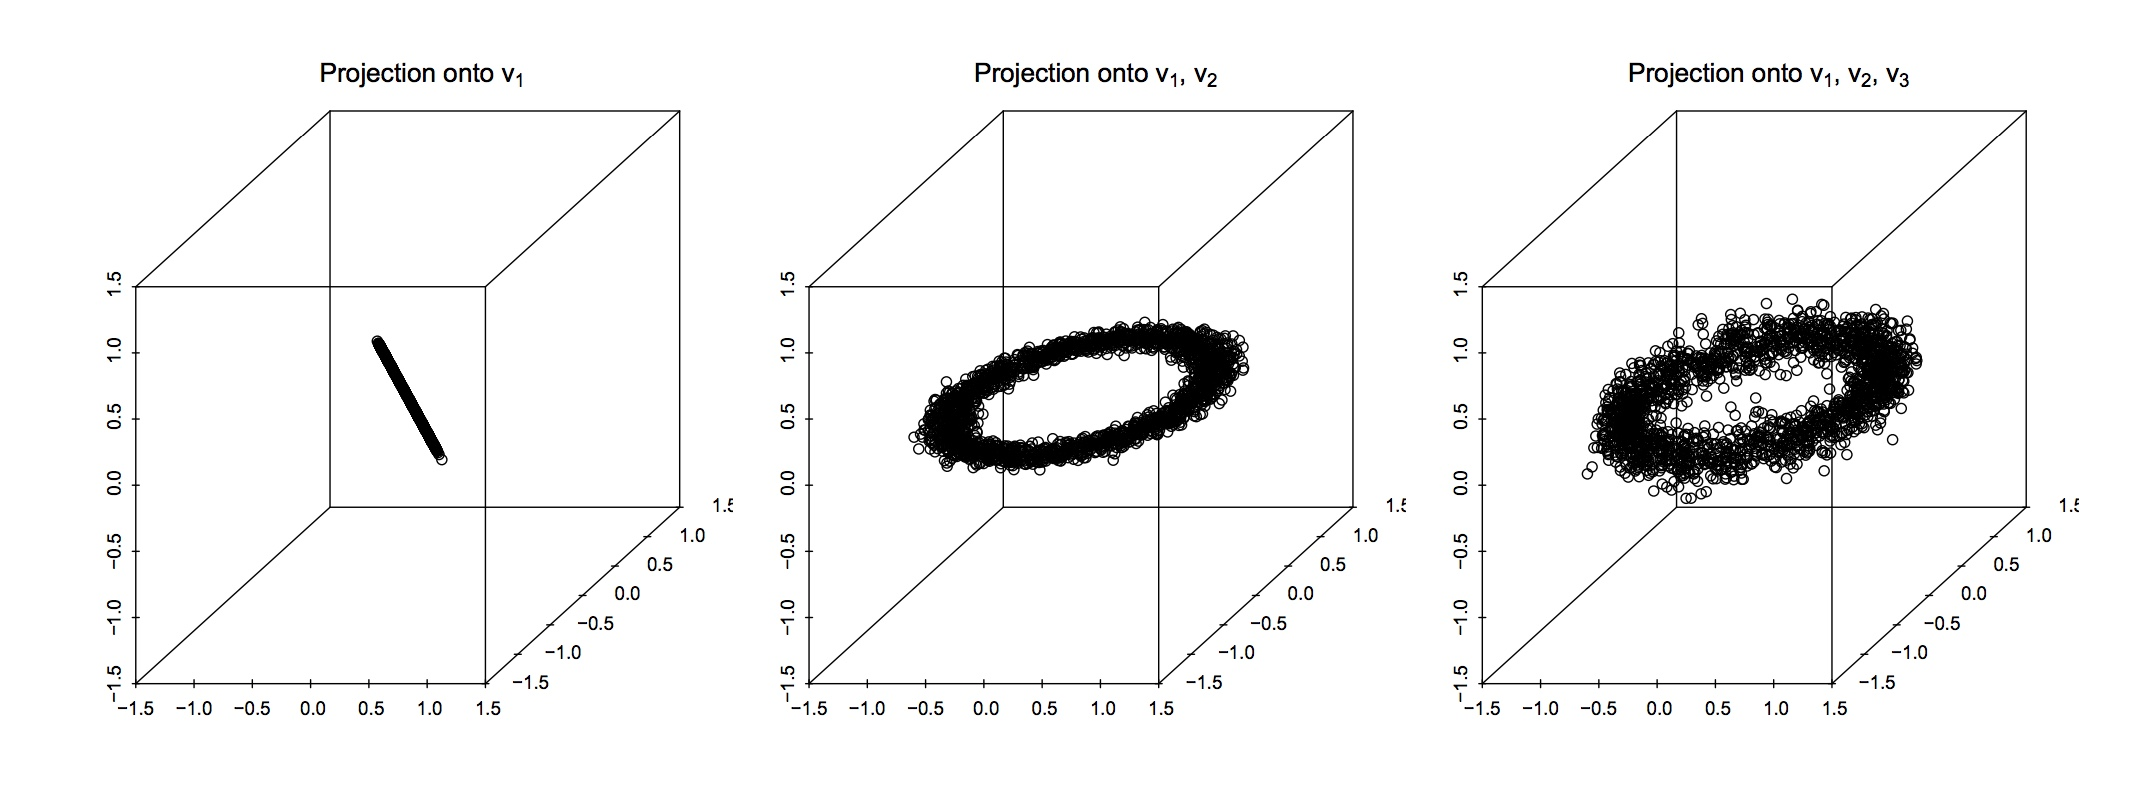
\includegraphics[height=2.5in]{pca_tib_2.jpeg}    
  \caption{(Source: CMU 36-462/36-662)}
\end{figure}
~\\
Now, let's generalize everything we've said to general $d$
and some given $k<d$. The dimension-reduced dataset 
$\left\{ U^\top \V{x}_1,\ldots,U^\top \V{x}_m \right\}\subset\R^k$ replaces each
point $\V{x}_i$ with its {\bf coordinates}. 
But we can still look at the {\bf projected} points - there are still points in
the original dimension $\R^d$. For example, each of these images is greyscale of
resolution $50$-by-$50$ pixels. So we can represent each image as a vector in
$\R^{50\times 50}=\R^{2500}$

\begin{figure}[H]
      \centering
      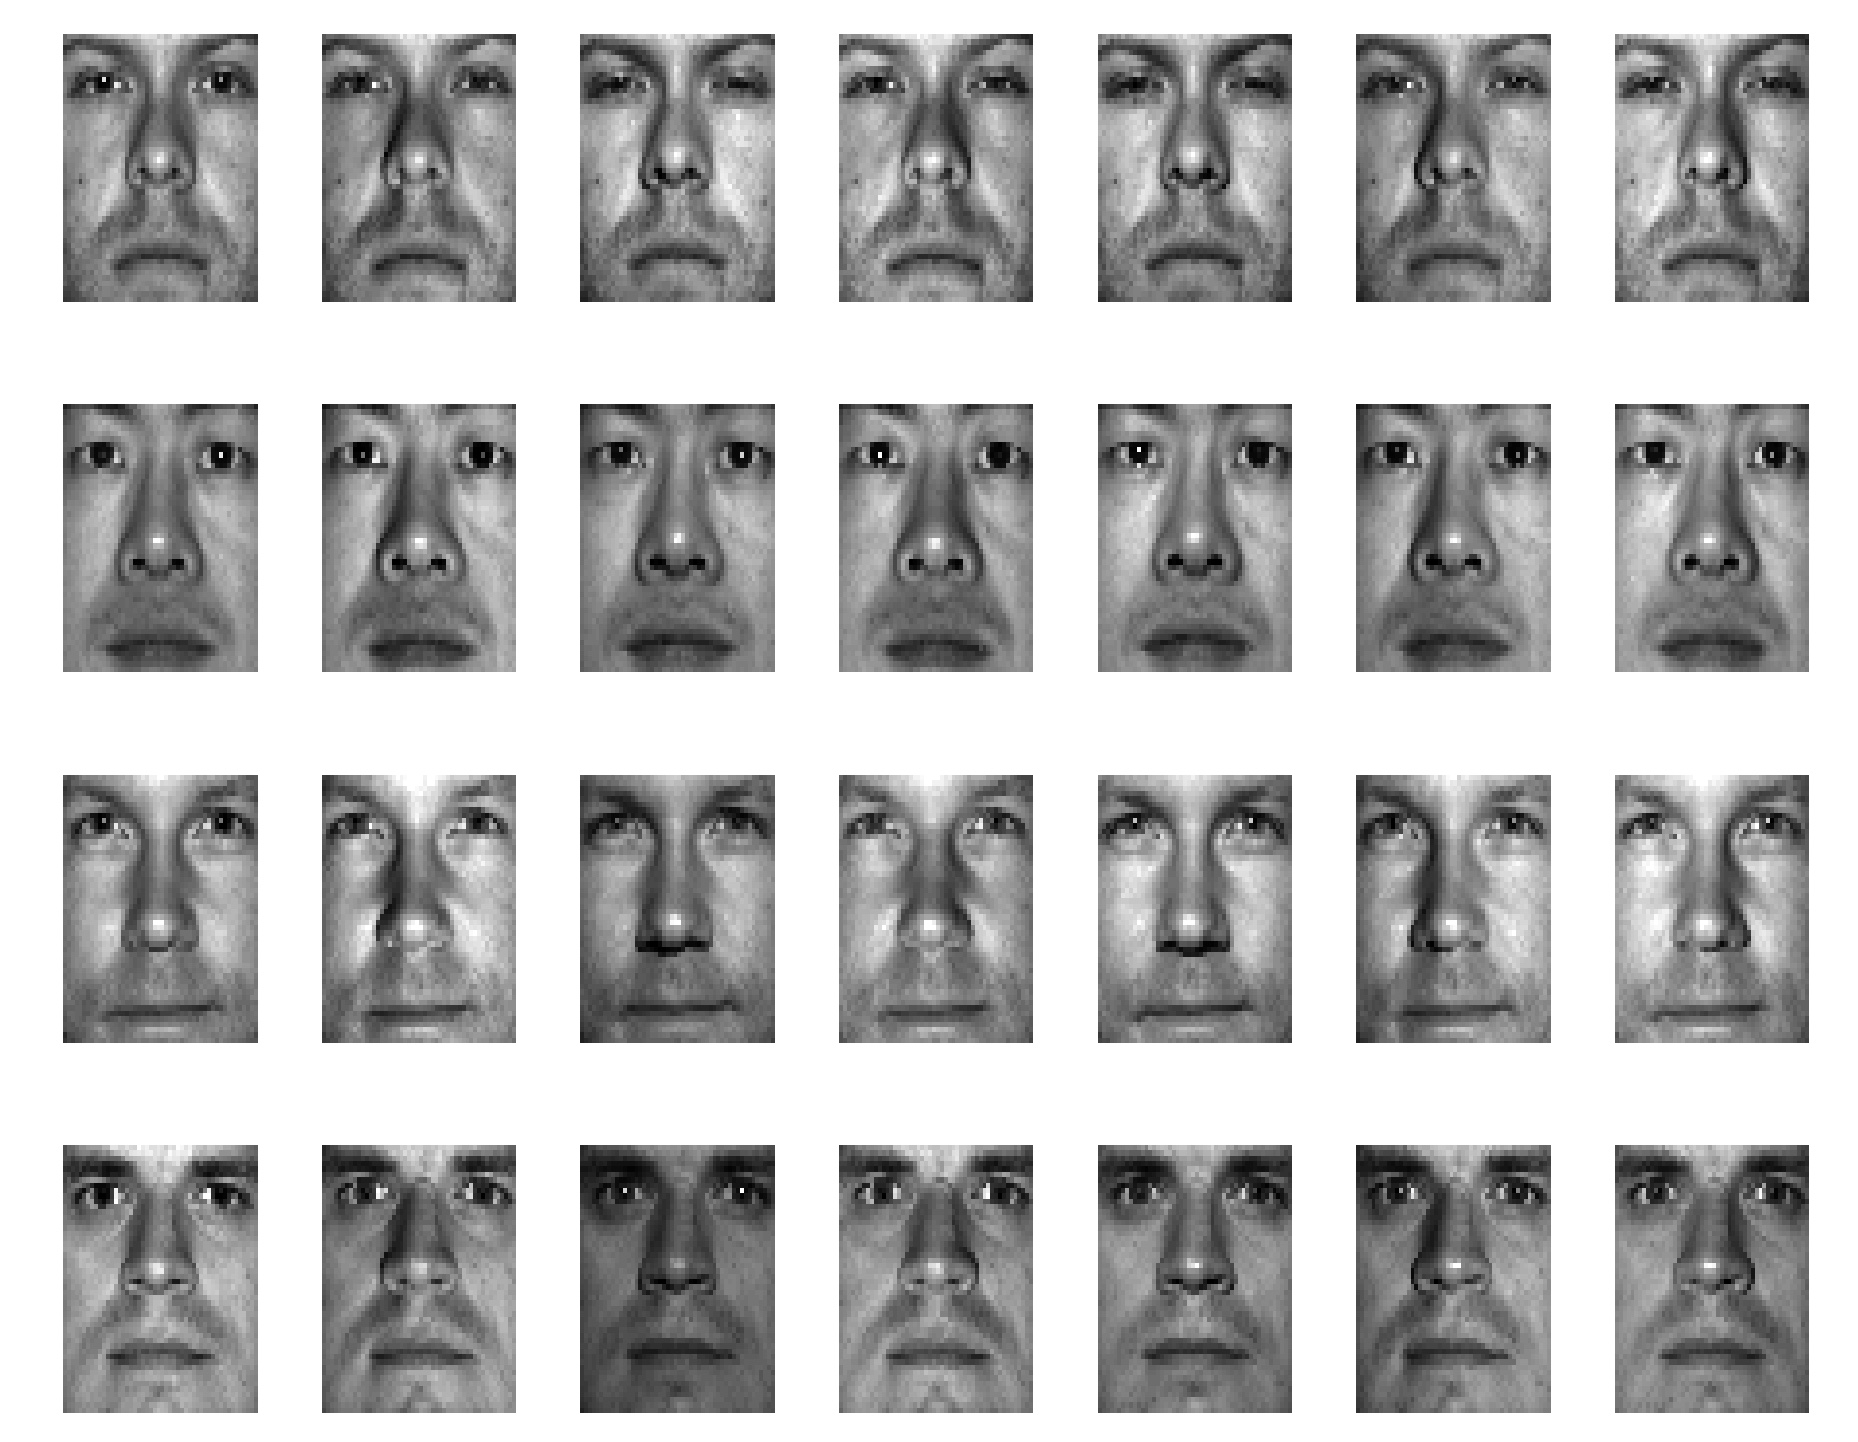
\includegraphics[height=2.7in]{pca_faces_before.jpeg}        
      \caption{Faces of four people from the Yale face dataset}
    \end{figure}
~\\
    Now we run PCA with $k=10$. In the dimension-reduced version
    each image is represented by a vector in $\R^{10}$. These are the {\bf
    coordinates.} We can't plot them as an image. But if we look at the {\bf
    projections}, which are still vectors in $\R^{2500}$ (that live on a
    $10$-dimensional subspace in $\R^{2500}$) we can plot them as images:
    %
\begin{figure}[H]
      \centering
      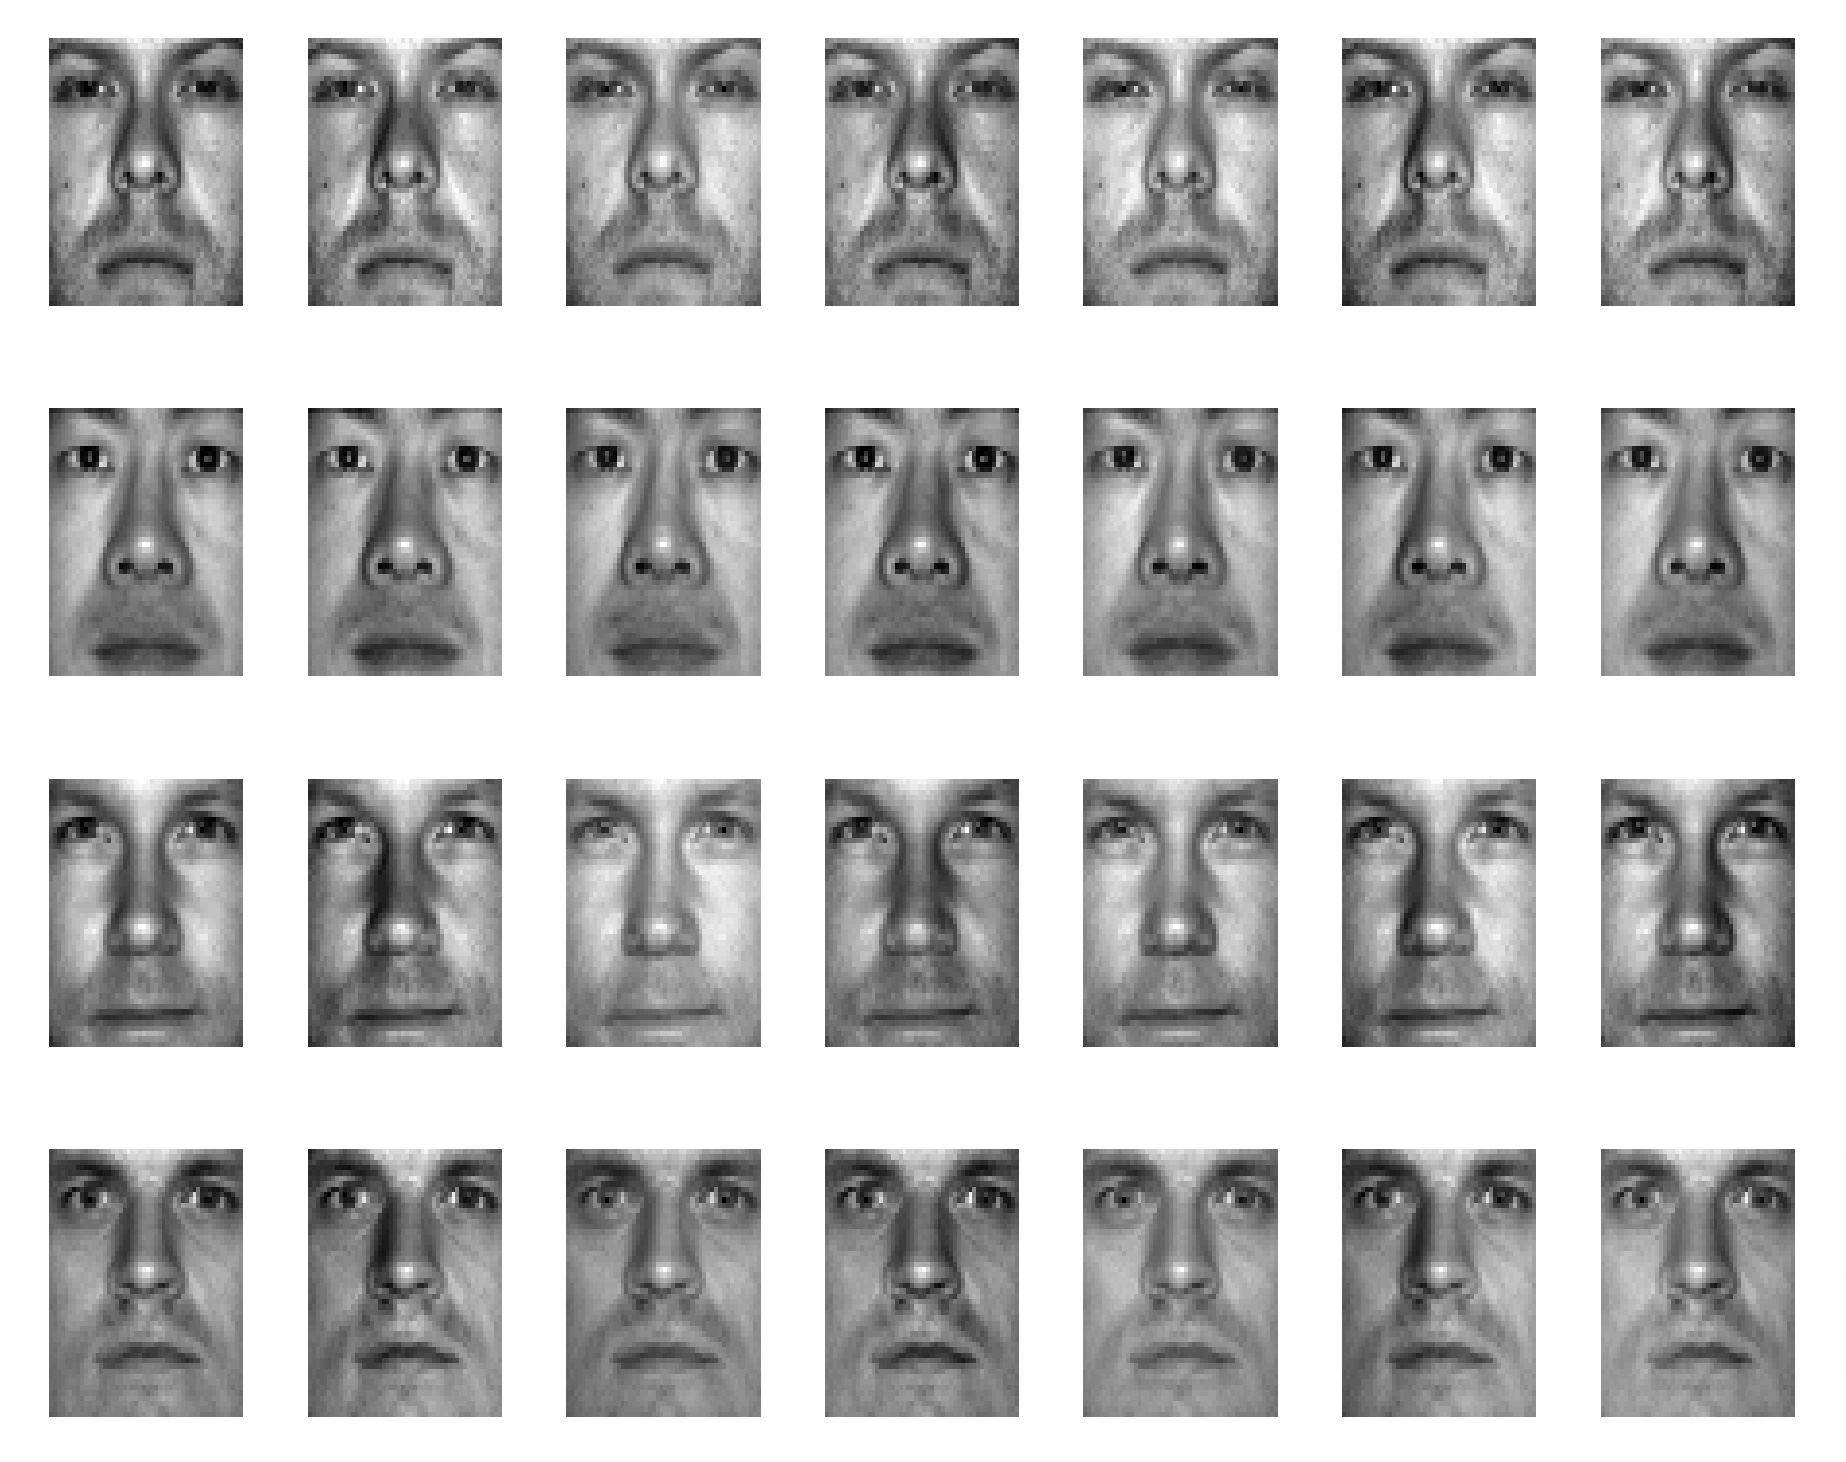
\includegraphics[height=2.7in]{pca_faces_after.jpeg}        
      \caption{Faces above projected to $10$ dimensional subspace found by PCA.
      Source: UML}
    \end{figure}
~\\
This is a simple form of {\bf compression}: to store the dimension-reduces
images, we need to store just $10$ principal vectors 
(each in $\R^{2500}$), and $m$ vectors in $\R^{10}$.
\\~\\
In contrast, if we were to look at the {\bf coordinates} in $\R^{10}$ we can't
plot them as images, but we can still hope that the dimension-reduced points of
images of same people stay together in $\R^{10}$. Here is a plot of the first
two coordinates of each image in this dataset:
\begin{figure}[H]
      \centering
      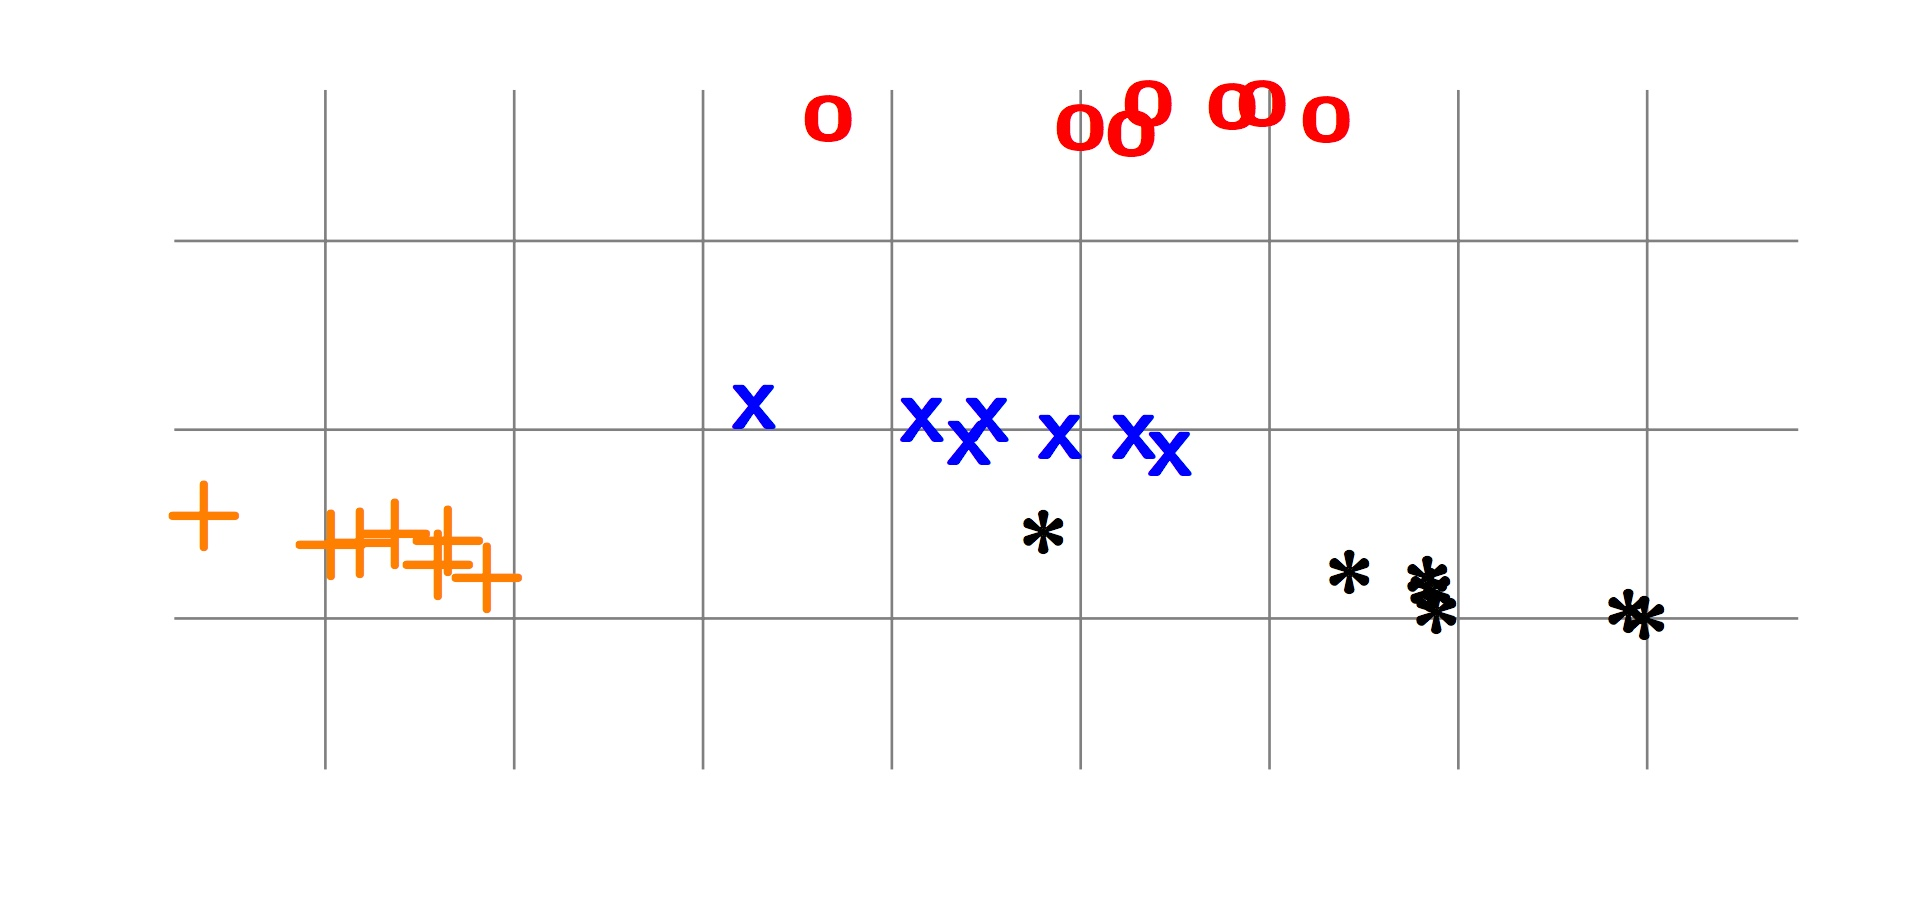
\includegraphics[height=2.7in]{pca_faces_proj.jpeg}        
      \caption{Faces above - dimension reduced to $2$. Each of
        the four people is marked with a different marker. (Source:
      UML)} 
    \end{figure}


\subsection{Interpreting and using the principal vectors as ``typical data
points''}

Interestingly, the principal vectors themselves are vectors in $\R^d$. 
So they have the same dimension as the datapoints $\V{x}_1,\ldots,\V{x}_m$. But
they are not datapoints. They are orthonormal vectors in $\R^d$, carefully
chosen such that the first $k$ vectors provide the best linear approximation of
dimension $k$ to the dataset. In this sense, they are ``typical'' datapoints,
maximally different from each other (since they are orthonormal). It is often
very interesting to see what they would represent as datapoints.
\\~\\
For example, in the digit dataset, suppose we only look at the digit ``3'' and
run PCA with $k=2$. Then we can write any digit ``3'' as a sum of the mean
$\overline{\V{x}}$, and the first two principal vectors:
\begin{figure}[H]
      \centering
      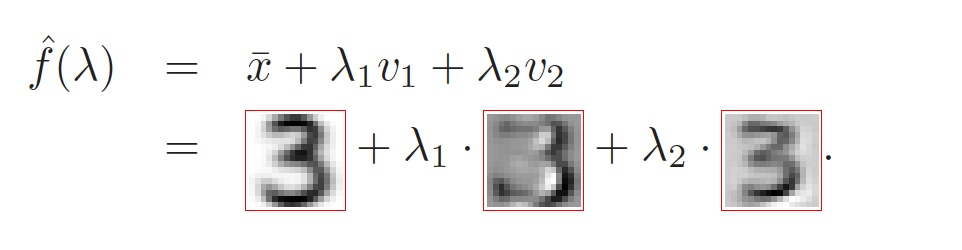
\includegraphics[height=1in]{3_pca_sum.jpeg}        
      \caption{Source: ESL}
    \end{figure}
~\\
The first principal component $\V{v}_1$ and the second principal component
$\V{v}_2$ are orthogonal and represent two maximally different 
``typical'' digit ``3''. They are {\bf not} digits in the dataset - they are
basis vectors. 
\\~\\
Another example: in the Yale face dataset, what would happen if we plot - as an
imgae - each the
leading principal vectors?
\begin{figure}[H]
      \centering
      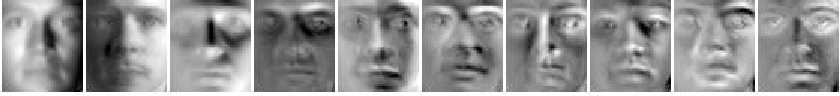
\includegraphics[width=6in]{yale_eigenfaces.png}        
      \caption{Source: Hao et al, Facial Recognition Using Tensor-Tensor
      Decompositions, SIAM Journal on Imaging Sciences 2013}
    \end{figure}
    %
    These are sometimes called ``eigenfaces''. Any image can
    written as a linear combination of these orthonormal vectors, and any image
    in the dataset can be writte - with small error - as a linear combination 
    {\bf of the first few.} So they represent maximally different 
    crucial features that appear in the faces in the dataset.



\subsection{Practical considerations.}

      \subsubsection{Fast computation of PCA}

  Recall that as machine learners we are also interested in numerical linear
  algebra, namely, algorithms that implement or linear algebra ideas in code
  efficiently and stably.
\\~\\
When $d\gg m$, so that we are working with a very high-dimensional dataset,
there is a good reason to try dimension reduction as part of our preprocessing.
However, exact diagonalization of the $d$-by-$d$ empirical covariance costs
$O(d^3)$. (This is a fact from numerical linear algebra you should remember.) So
if $d$ is huge, $O(d^3)$ can be a prohibitively expensive computation. 
When $d$ is large and $d\gg m$ we can use a nice trick and calculate the
eigenvectors of an $m$-by-$m$ matrix instead. This costs $O(m^3)$. The 
following algorithm calculates PCA in the cost of $O(m^2\cdot d)$ (see UML
23.1.1). 
Here is how
you should remember it: our data matrix $X$ (remember linear regression and
logistic regression?) is $m$-by-$d$, and PCA costs order of 
$(small)^2\cdot(large)$ steps. 



  \begin{myalgo}{PCA}
\textbf{input}~ \+ \\
A matrix of $m$ examples $X \in \reals^{m,d}$  \\
number of components $n$ \- \\
\textbf{if} $(m > d)$ \+ \\
    $A = X^\top X$ \\ 
    Let $\u_1,\ldots,\u_n$ be the eigenvectors of $A$ with largest eigenvalues \- \\
\textbf{else} \+ \\
    $B = X X^\top$ \\
    Let $\v_1,\ldots,\v_n$ be the eigenvectors of $B$ with largest
    eigenvalues \\
    for $i=1,\ldots,n$ set $\u_i = \frac{1}{\|X^\top
      \v_i\|} \, X^\top \v_i$ \- \\
\textbf{output}: $\u_1,\ldots,\u_n$ 
\end{myalgo}


\subsubsection{Choosing $k$}

In practice, no one tells us the dimension $k$ to which we should reduce. 
How shall we choose $k$? If we choose $k$ too high, we are ``wasteful'' in that
we don't need so many dimensions. If we choose $k$ too low, we throw away
essential parts of the data, so that the dimension-reduced dataset does not
capture the essential features of the dataset.
\\~\\
Let's begin by a noticing that PCA tells us when the data sits 
{\bf exactly} on a
$k$-dimensional linear subspace of $\R^d$. 
\\~\\
{\bf Exercise.} 
Suppose that our training sample $\V{x}_1,\ldots,\V{x}_m$ is contained in a
subspace $V\subset \R^d$, with $dim(V)=k$. Let $S$ be the $d$-by-$d$
 empirical covariance
 matrix of the training sample. Show that $rank(S)\leq k$.
\\~\\ 
 This means that if indeed the training sample lies exactly on a $k$-dimension
 linear subspace of $\R^d$, then we will have $k$ nonzero principal values
 (recall that the principal values are just the eigenvalues of the empirical
 covariance $S$) and the rest will be zero. 
\\~\\
Now imagine that the training sample lies close to such a subspace. What would
happen? You guessed correctly - we will have $k$ large principal values, and he
rest will be non-zero but small. (Recall that we've seen something like this in
linear regression.) So the best way to choose $k$ from the data would be somehow
related to finding how many ``large'' principal values there are. We don't
discuss a formal algorithm for choosing $k$, but this is the general idea.
The most popular informal method (which is not in fact an algorithm) involves
plotting the principal components in decreasing order simply over their index,
and making an ``intuitive guess'' about the number of ``large'' principal
values. This number is chosen to be $k$. Such a plot is sometimes called a
``Scree Plot''. 
\begin{figure}[H]
      \centering
      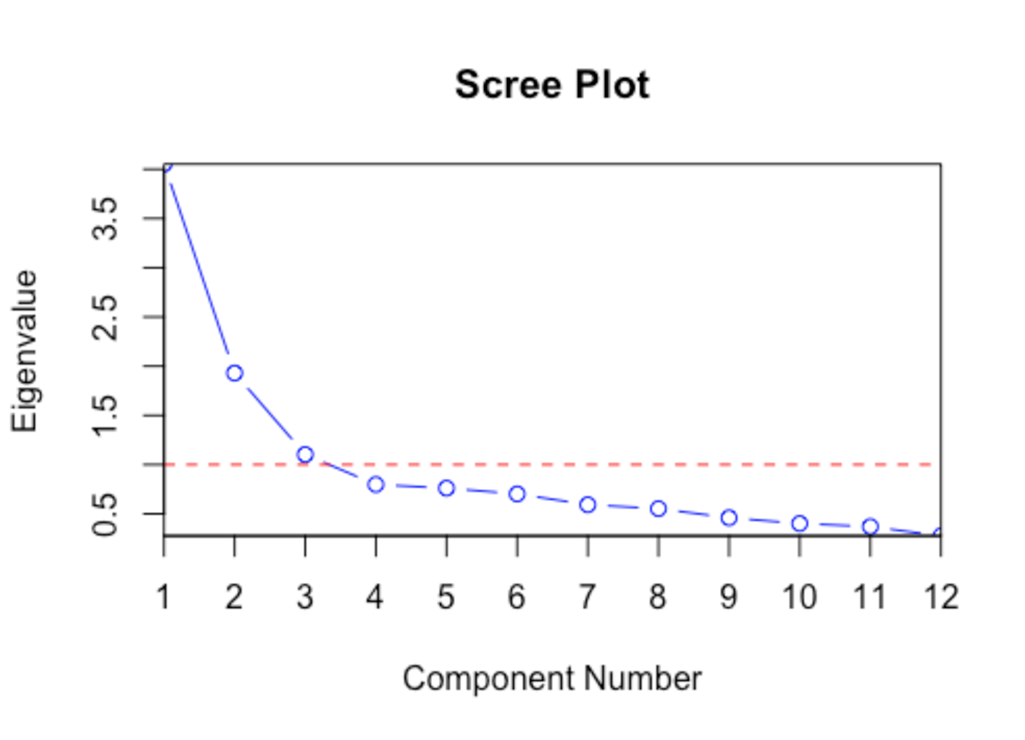
\includegraphics[height=2.7in]{screeplot.pdf}        
      \caption{Typical plot of principal components over their index. (Source:
      Wikipedia)}
    \end{figure}
~\\
{\bf Exercise.} Write a simulation to observe this phenomenon. In your
simulation, start with data in $\R^d$ that lie exactly on a $k$-dimensional
linear subspace of $\R^d$, and plot the principal values. Now move the data
slightly away from the subspace and plot the principal values. 

\section{Clustering}

To get another taste of an unsupervised learning problem, let's look at {\bf
clustering.} We are given
an unlabeled training sample $\V{x}_1,\ldots,\V{x}_m$ and wish to partition 
the $m$ points into $k$ sets, or {\bf clusters.} Sometimes we have a clear idea
of what $k$ should be (how many clusters we should be looking for), and
sometimes we have to figure out $k$ ourselves based on the data.

Why cluster?
\begin{itemize}
  \item Clustering partitions the dataset into subsets of ``similar'' points. As
    an exploratory step, we might be interested in what are the common
    properties of each cluster found by out clustering algorithm.
  \item We may want to validate an existing partition someone gave us, and see
    if an unsupervised clustering algorithm (which uses no labels and no
    knowledge other than the points themselves) produces the same partition.
\end{itemize}

Note that there are no labels for us to use. This means that, unlike supervised
classification, {\bf there is no ground truth}. (Compare this to the opposite
  situation - in supervised classification, under the realizability assumption,
there was a ``ground truth'' function $f$ we were trying to predict.) 
Therefore, clustering is not a
well-defined problem with a single answer. For example, the following dataset in
$\R^2$ 
\begin{figure}[H]
      \centering
      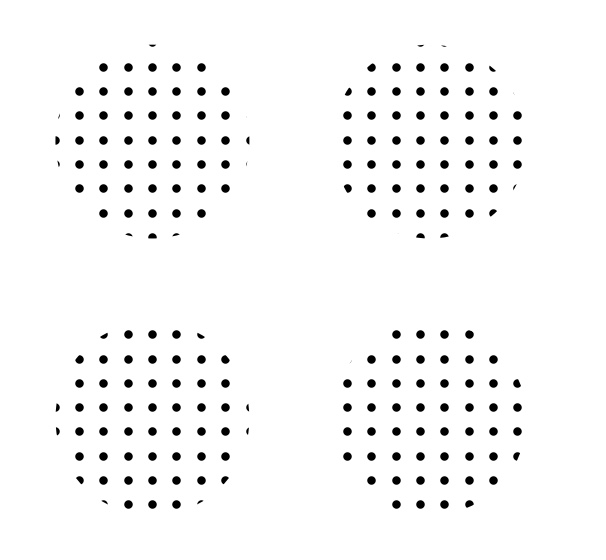
\includegraphics[height=2.7in]{cluster0.jpeg}        
      \caption{(Source: Shai Shalev-Shwartz slides)}
    \end{figure}
%
    can be clustered like this
    \begin{figure}[H]
      \centering
      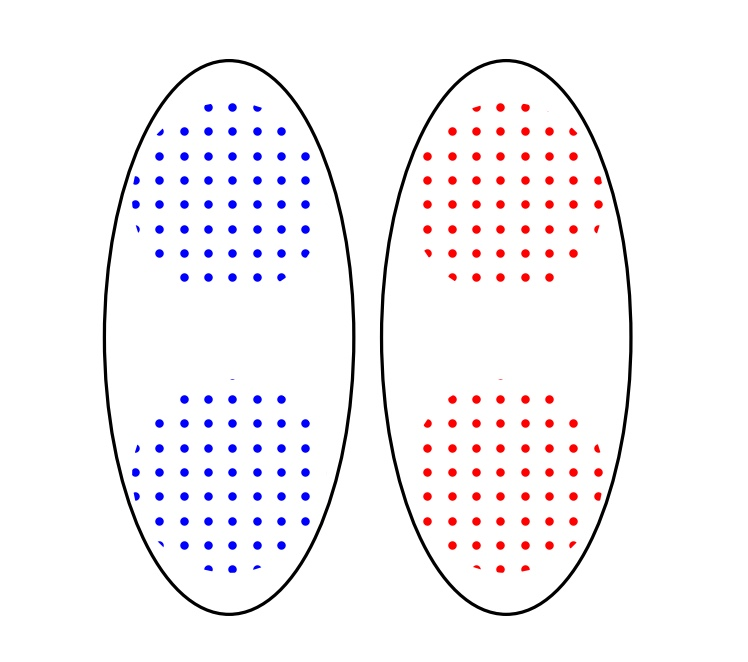
\includegraphics[height=2.7in]{cluster1.jpeg}        
      \caption{(Source: Shai Shalev-Shwartz slides)}
    \end{figure}
%
    or like this
    \begin{figure}[H]
      \centering
      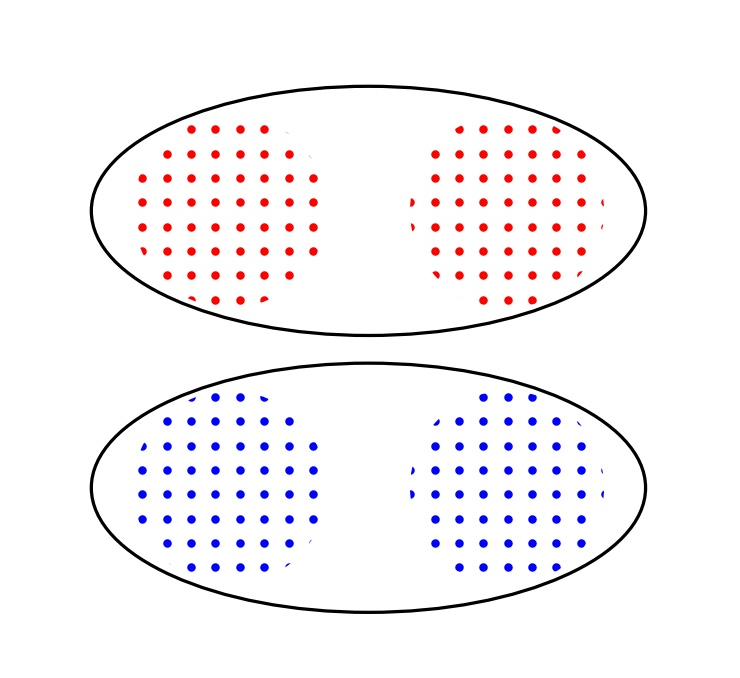
\includegraphics[height=2.7in]{cluster2.jpeg}        
      \caption{(Source: Shai Shalev-Shwartz slides)}
    \end{figure}

    Even though the problem is not well-defined, 
    we can nonetheless develop a systematic approach to clustering.
    This systematic approach can be defined on any sample space, not just
    $\R^d$: 
    \\\~\\
    Assume we have a distance measure (a metric) on our sample space. 
    (For example, if $\X=\R^d$ we may consider the Euclidean norm
    and take $d(\V{x}_1,\V{x}_2) = \norm{\V{x}_1-\V{x}_2}$.) 
    \begin{itemize}
      \item Definition: A clustering of the dataset $\{ \V{x}_1,\ldots,\V{x}_m \}$
        into $k$ clusters is simply a 
        partition $\{ \V{x}_1,\ldots,\V{x}_m \}=\biguplus_{j=1}^k C_j$
      \item Define a {\bf cost function} for this clustering: 
       \[
         G(C_1,\ldots,C_k) = \min_{\mu_1,\ldots,\mu_k\in\R^d} 
         \sum_{j=1}^k
         \sum_{\V{x}\in C_j} d(\V{x},\mu_j)^2
       \]
     \item 
       The quantity 
        \[ 
          \text{argmin}_{\mu_j\in\R^d}  \sum_{\V{x}\in C_j} d(\V{x},\mu_j)^2
        \]
       is called the {\bf centroid} of cluster $C_j$. 

       
         \end{itemize}

   {\bf Exercise.} 
   Assume $\X=\R^d$ and $d$ is the Euclidean norm.
   Show that the centroid of a set $C_j$ is simply the average
   \[
     \mu_j := \frac{1}{|C_j|} \sum_{\V{x}\in C_j} \V{x}\,.
            \]
          The quantity $\mu_j$ 
          has a name in Mechanics. How is it called? It has a name in
          Statistics. How is it called? The quantity 
          $\sum_{\V{x}\in C_j} d(\V{x},\mu_j)^2$ has a name in Mechanics. How is
          it called? It has a name in Statistics. How is it called?
\\~\\ How do we find the minimum of $G$?
   Fix $k$. The objective function $G$ is  a {\bf function of partitions}:
   minimizing it would navigating the space of all possible partitions of $m$
   objects into $k$ subsets. (How many are there?)
   Not surprisingly, it can be shown that minimizing the cost 
   function $G$ is NP-hard, and we must resort to heuristics. 
   The most famous heuristic for minimizing $G$ is an iterative algorithm known
   as {\bf $k$-means clustering.}

\subsection{k-means}

$k$-means clustering uses {\bf Lloyd's Algorithm}, a heuristic approach that
attempts to 
minimize $G$. Let's assume for simplicity that $\X=\R^d$ and the distance
function $d$ is just the Euclidean norm. (This heuristic can be adapted to
other spaces as well.)
        \begin{itemize}
          \item Input: Set $\V{x}_1,\ldots,\V{x}_m$ and number of clusters $k$
          \item Step 0. Choose initial centroids $\mu_1,\ldots,\mu_k$
          \item Repeat until convergence: \\
            (i) set $C_j$ to be the points
            $\V{x}_i$ closer to $\mu_j$ than to any other centroid. \\(ii) update 
            $\mu_j$ the centroid of $C_j$, which as you showed in the exercise
            above, is simply 
            \[
              \mu_j := \frac{1}{|C_j|} \sum_{\V{x}\in C_j} \V{x}
            \]

        \end{itemize}

What's going on here? 
If we choose the centroids, this induces a simple partition of the dataset -
each point is associated to a subset according to its nearest centroid. (These
  subsets are 
called {\bf Voronoi cells.}) And if we choose a partition, we define the
centroids as the subset averages. 
\\~\\
So Lloyd's algorithm is an iterative {\bf alternating} algorithm. 
We start from some initial
guess of the centroids, then use them to induce a partition, then use this
partition to define centroids, and so on. We hope that the algorithm converges;
we hope that won't be too sensitive to the initial choice of centroids.
\\~\\
Here is an example in  $d=2$ dimensions, on $m=300$ points, and we cluster into
$k=3$ clusters: 
\begin{figure}[H]
      \centering
      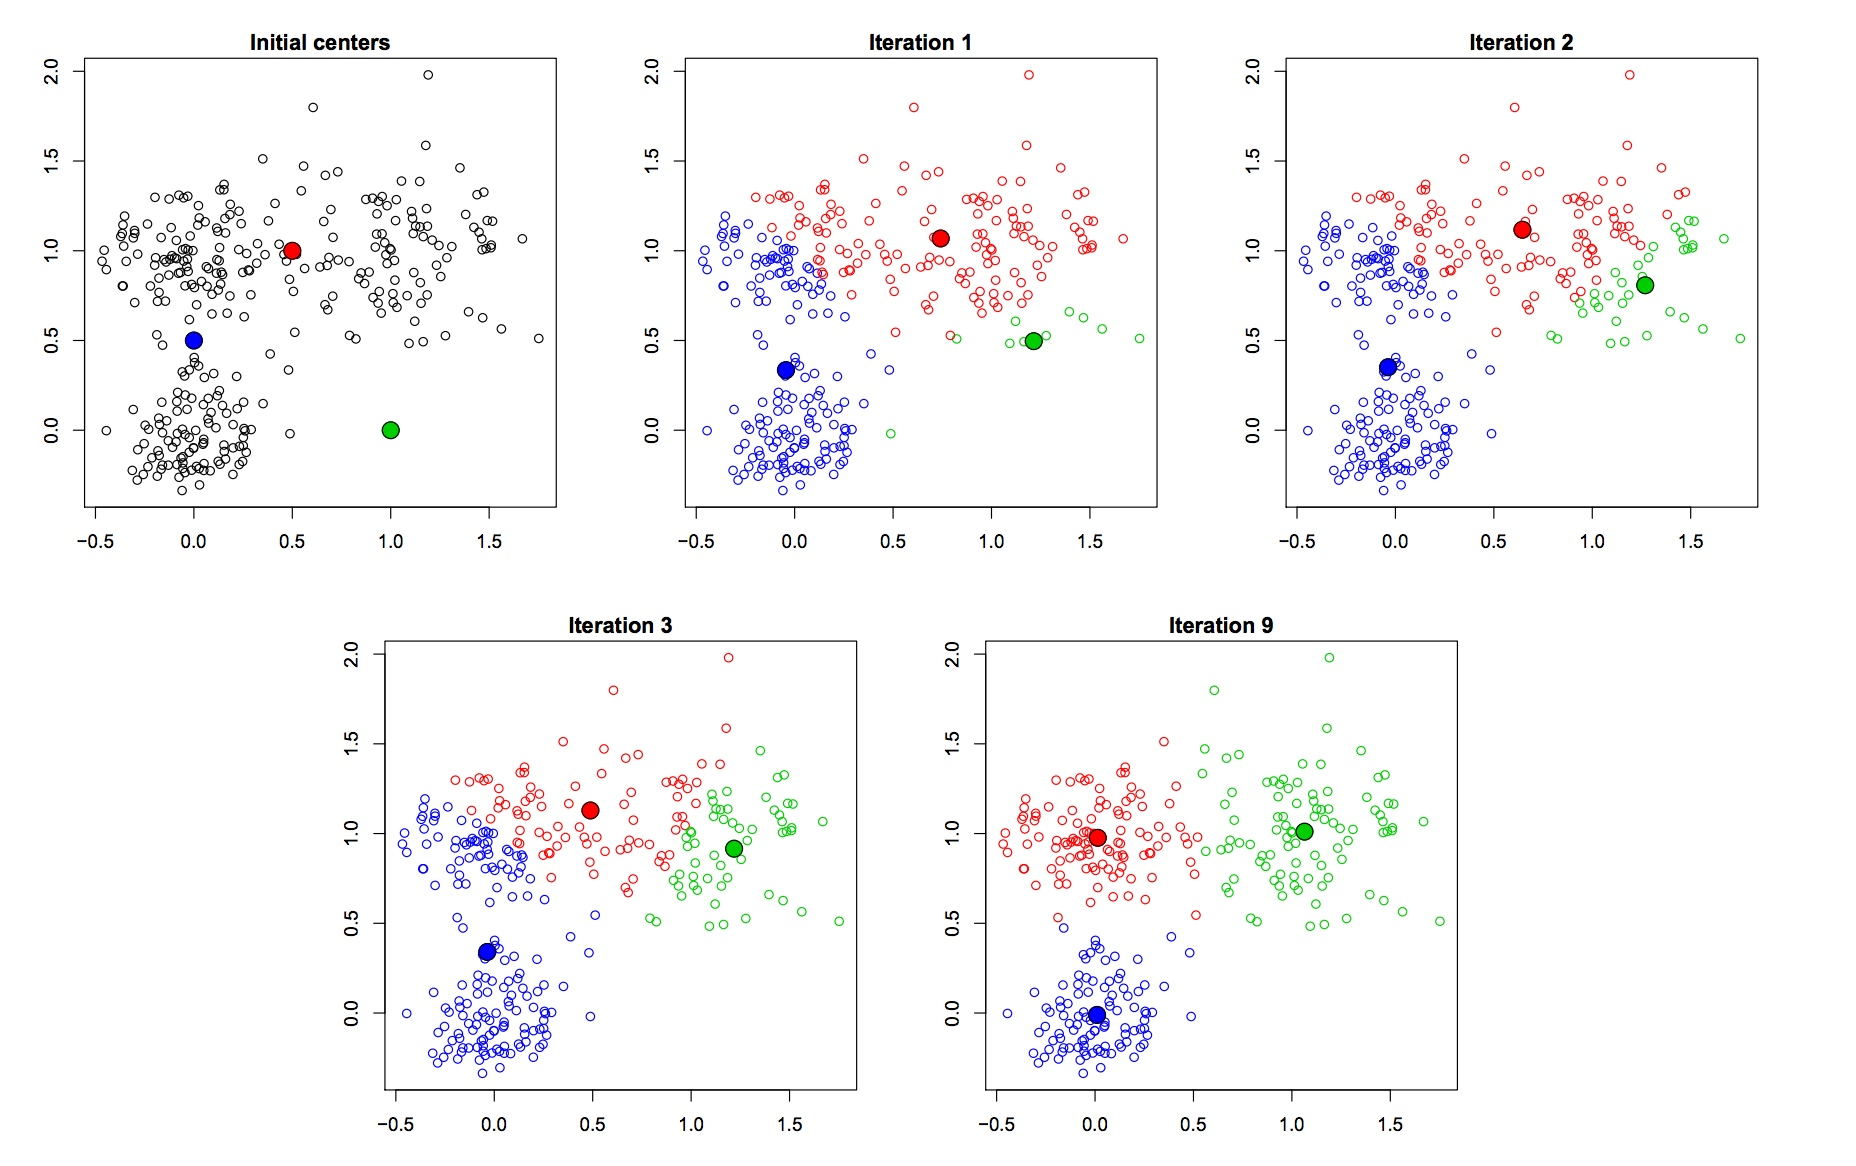
\includegraphics[height=3.5in]{kmeans.jpeg}        
      \caption{(Source: CMU 36-462/36-662)}
    \end{figure}
~\\ 
Here are some properties of Lloyd's algorithm, which we won't prove. You are
encouraged to play with them in simulation and observe them:
    \begin{itemize}
        \item Variation within each cluster always decreases from iteration to
          iteration.
        \item The algorithm always converges - but may converge very slowly.
        \item The end result can drastically depend on the initialization.
          In other words, the algorithm converges to a local minimum of the
          function $G$ which depends on the initial choice of centroids. 
        \end{itemize}

~\\Here is an example using the same dataset as in the image above. This
        time we specify $k=4$. Each panel has different initial conditions:

  \begin{figure}[H]
      \centering
      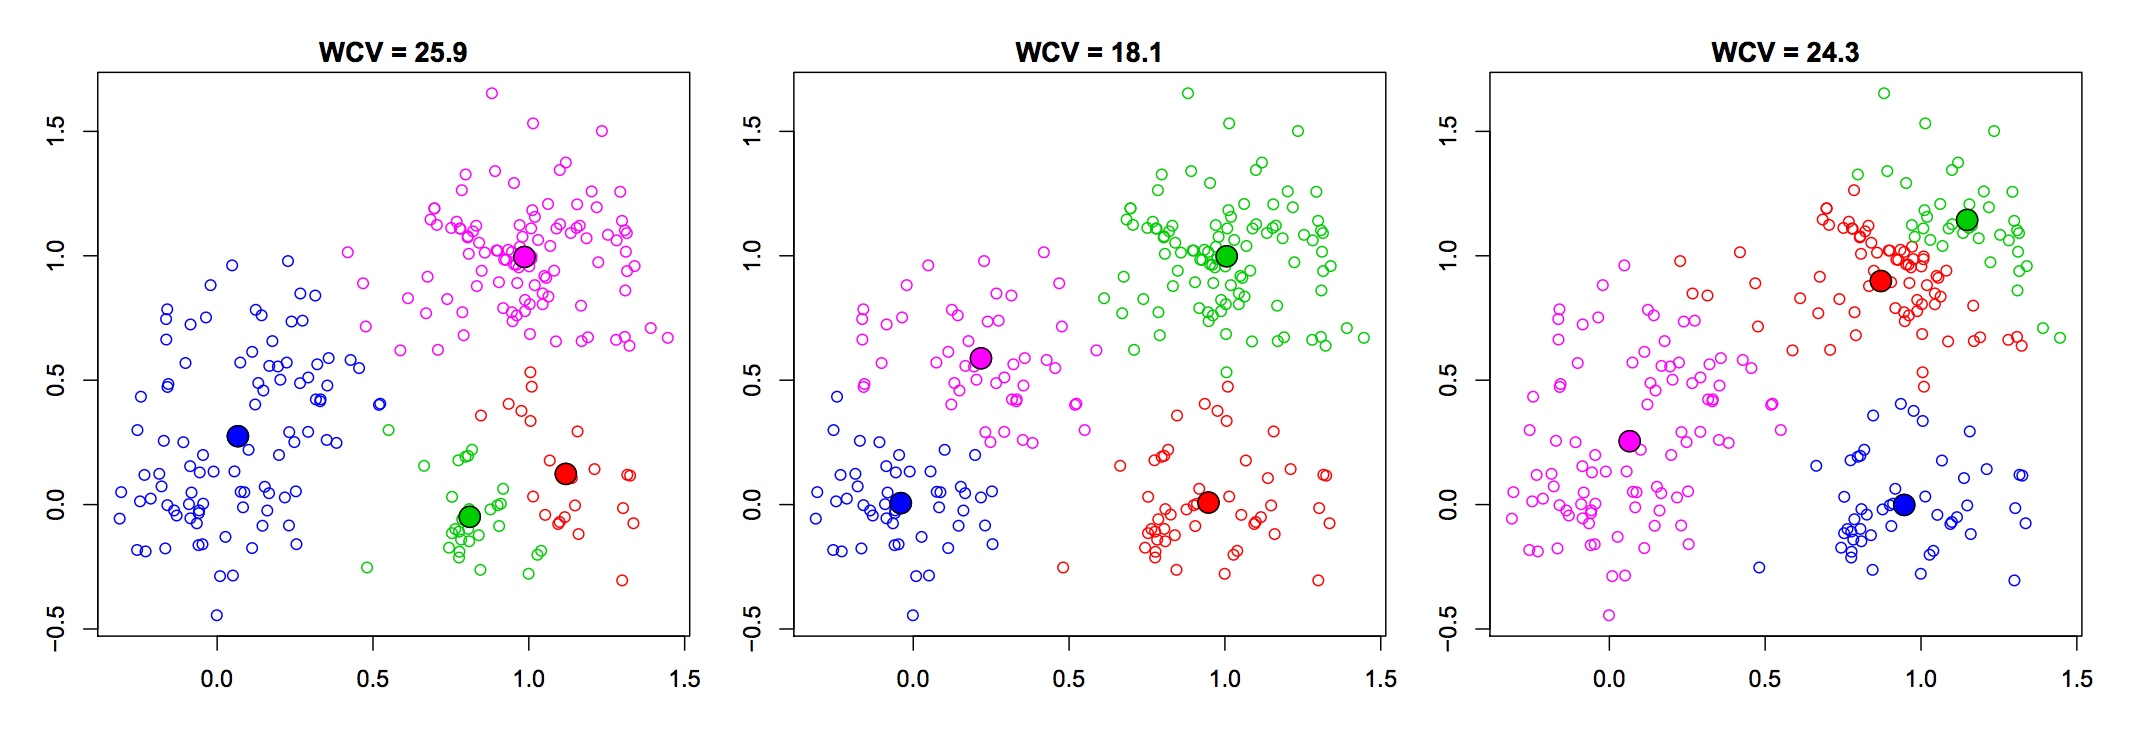
\includegraphics[height=2in]{kmeans_iter.jpeg}        
      \caption{(Source: CMU 36-462/36-662)}
    \end{figure}
~\\
Since we are attempting to minimize the global cost function $G$, one
    way to handle the dependence on initial conditions is to run the algorithm a few times and take the result which
    achieved lowest cost.
\\~\\
Finally, how do we choose the number of clusters $k$? In fact $k$ is a
bias-variance parameter. The higher $k$ (the more subsets we take) the lower the
value of $G$ we will obtain. This is analogous to overfitting in supervised
learning as we increase the complexity of the model:
\begin{figure}[H]
      \centering
      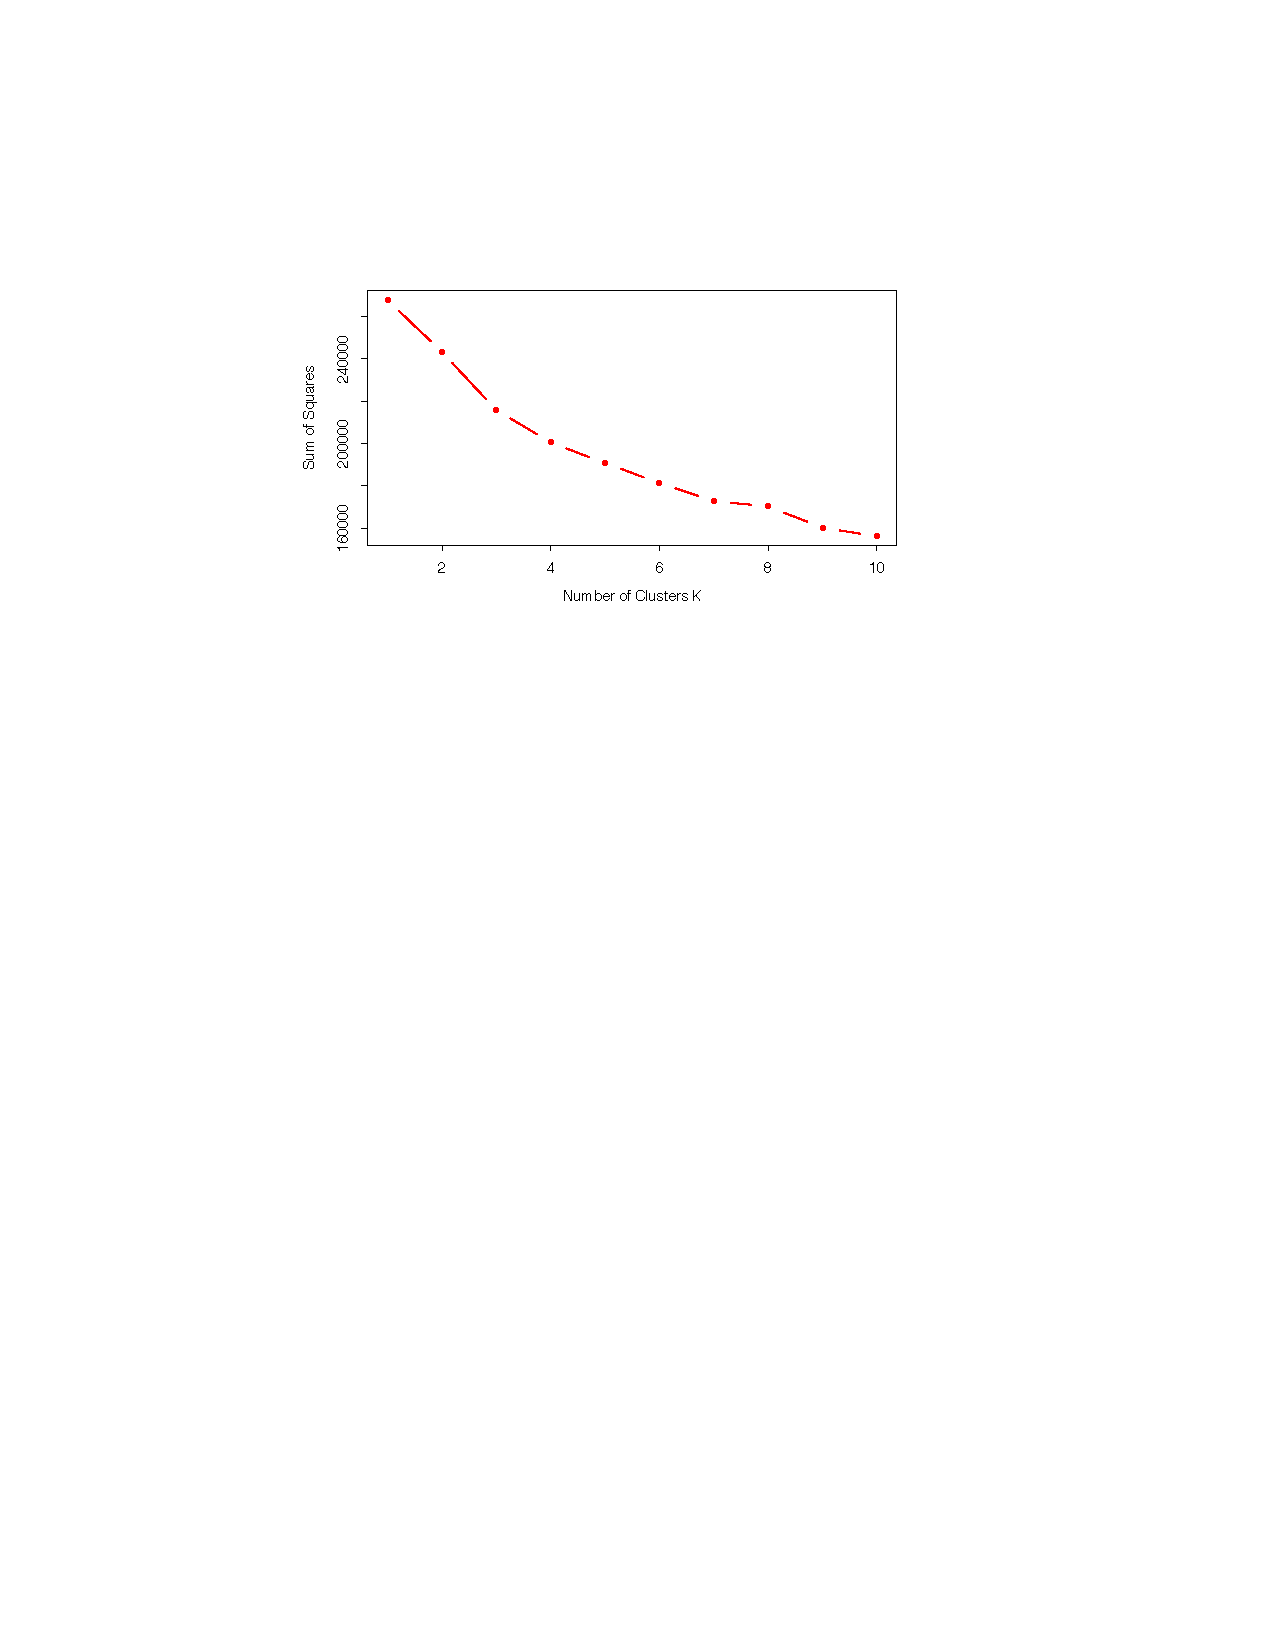
\includegraphics[height=2.4in]{kmeans_k_ss.pdf}        
      \caption{Source: ESL}
    \end{figure}







